\documentclass[11pt, preprint]{aastex}
\usepackage{amsmath}
\usepackage{natbib}
\setcitestyle{numbers}

\begin{document}
\title{Data Management Applications Design}
\slugcomment{Aug 4, 2011}
\author{Tim Axelrod}
\author{Jacek Becla}
\author{Gregory Dubois-Felsmann}
\author{Jeff Kantor}
\author{Kian-Tat Lim}
\author{Robert Lupton}

\section{Introduction}

The LSST Science Requirements Document \citep{SRD} specifies a set of
science goals to be achieved from the LSST observing program.  To
enable the achievement of these goals, the LSST Data Management System
(``DMS'') is required to generate, or enable the generation of, a set
of data products, and to make them available to scientists and the
public. To carry out this mission the DMS performs the following major
functions:

\begin{itemize}
\item Processes the incoming stream of images generated by the camera
  system during observing to produce transient alerts and to archive
  the raw images.

\item Roughly once per year, creates and archives a Data Release (``DR''),
  which is a static self-consistent collection of data products
  generated from all survey data taken from the date of survey
  initiation to the cutoff date for the Data Release. The data
  products include optimal measurements of the properties (shapes,
  positions, fluxes, motions) of all
  objects, including those below the single visit sensitivity limit,
  astrometric and photometric calibration of the full survey object
  catalog, and limited classification of objects based on both their
  static properties and time-dependent behavior.  Deep coadded images
  of the full survey area are produced as well.

\item Periodically creates new calibration data products, such as bias
  frames and flat fields, that will be used by the other processing
  functions.

\item Makes all LSST data available through an interface that
  utilizes, to the maximum possible extent, community-based standards
  such as those being developed by the Virtual Observatory (``VO''), and
  facilitates user data analysis and the production of user-defined
  data products at Data Access Centers (``DAC'') and at external sites.
\end{itemize}

The overall architecture of the DMS is shown in Fig. 1.  This document
discusses the role of the Applications layer in the first three
functions listed above.  The fourth is discussed separately in the SUI
Conceptual Design \citep{SUI}.  The overall architecture of the DMS is
discussed in more detail in the Data Management System Design document
\citep{DMSSystem}. The DMS requirements are described in detail in the
Data Management Subsystem Requirements document \citep{DMSFRS}.

\begin{figure}
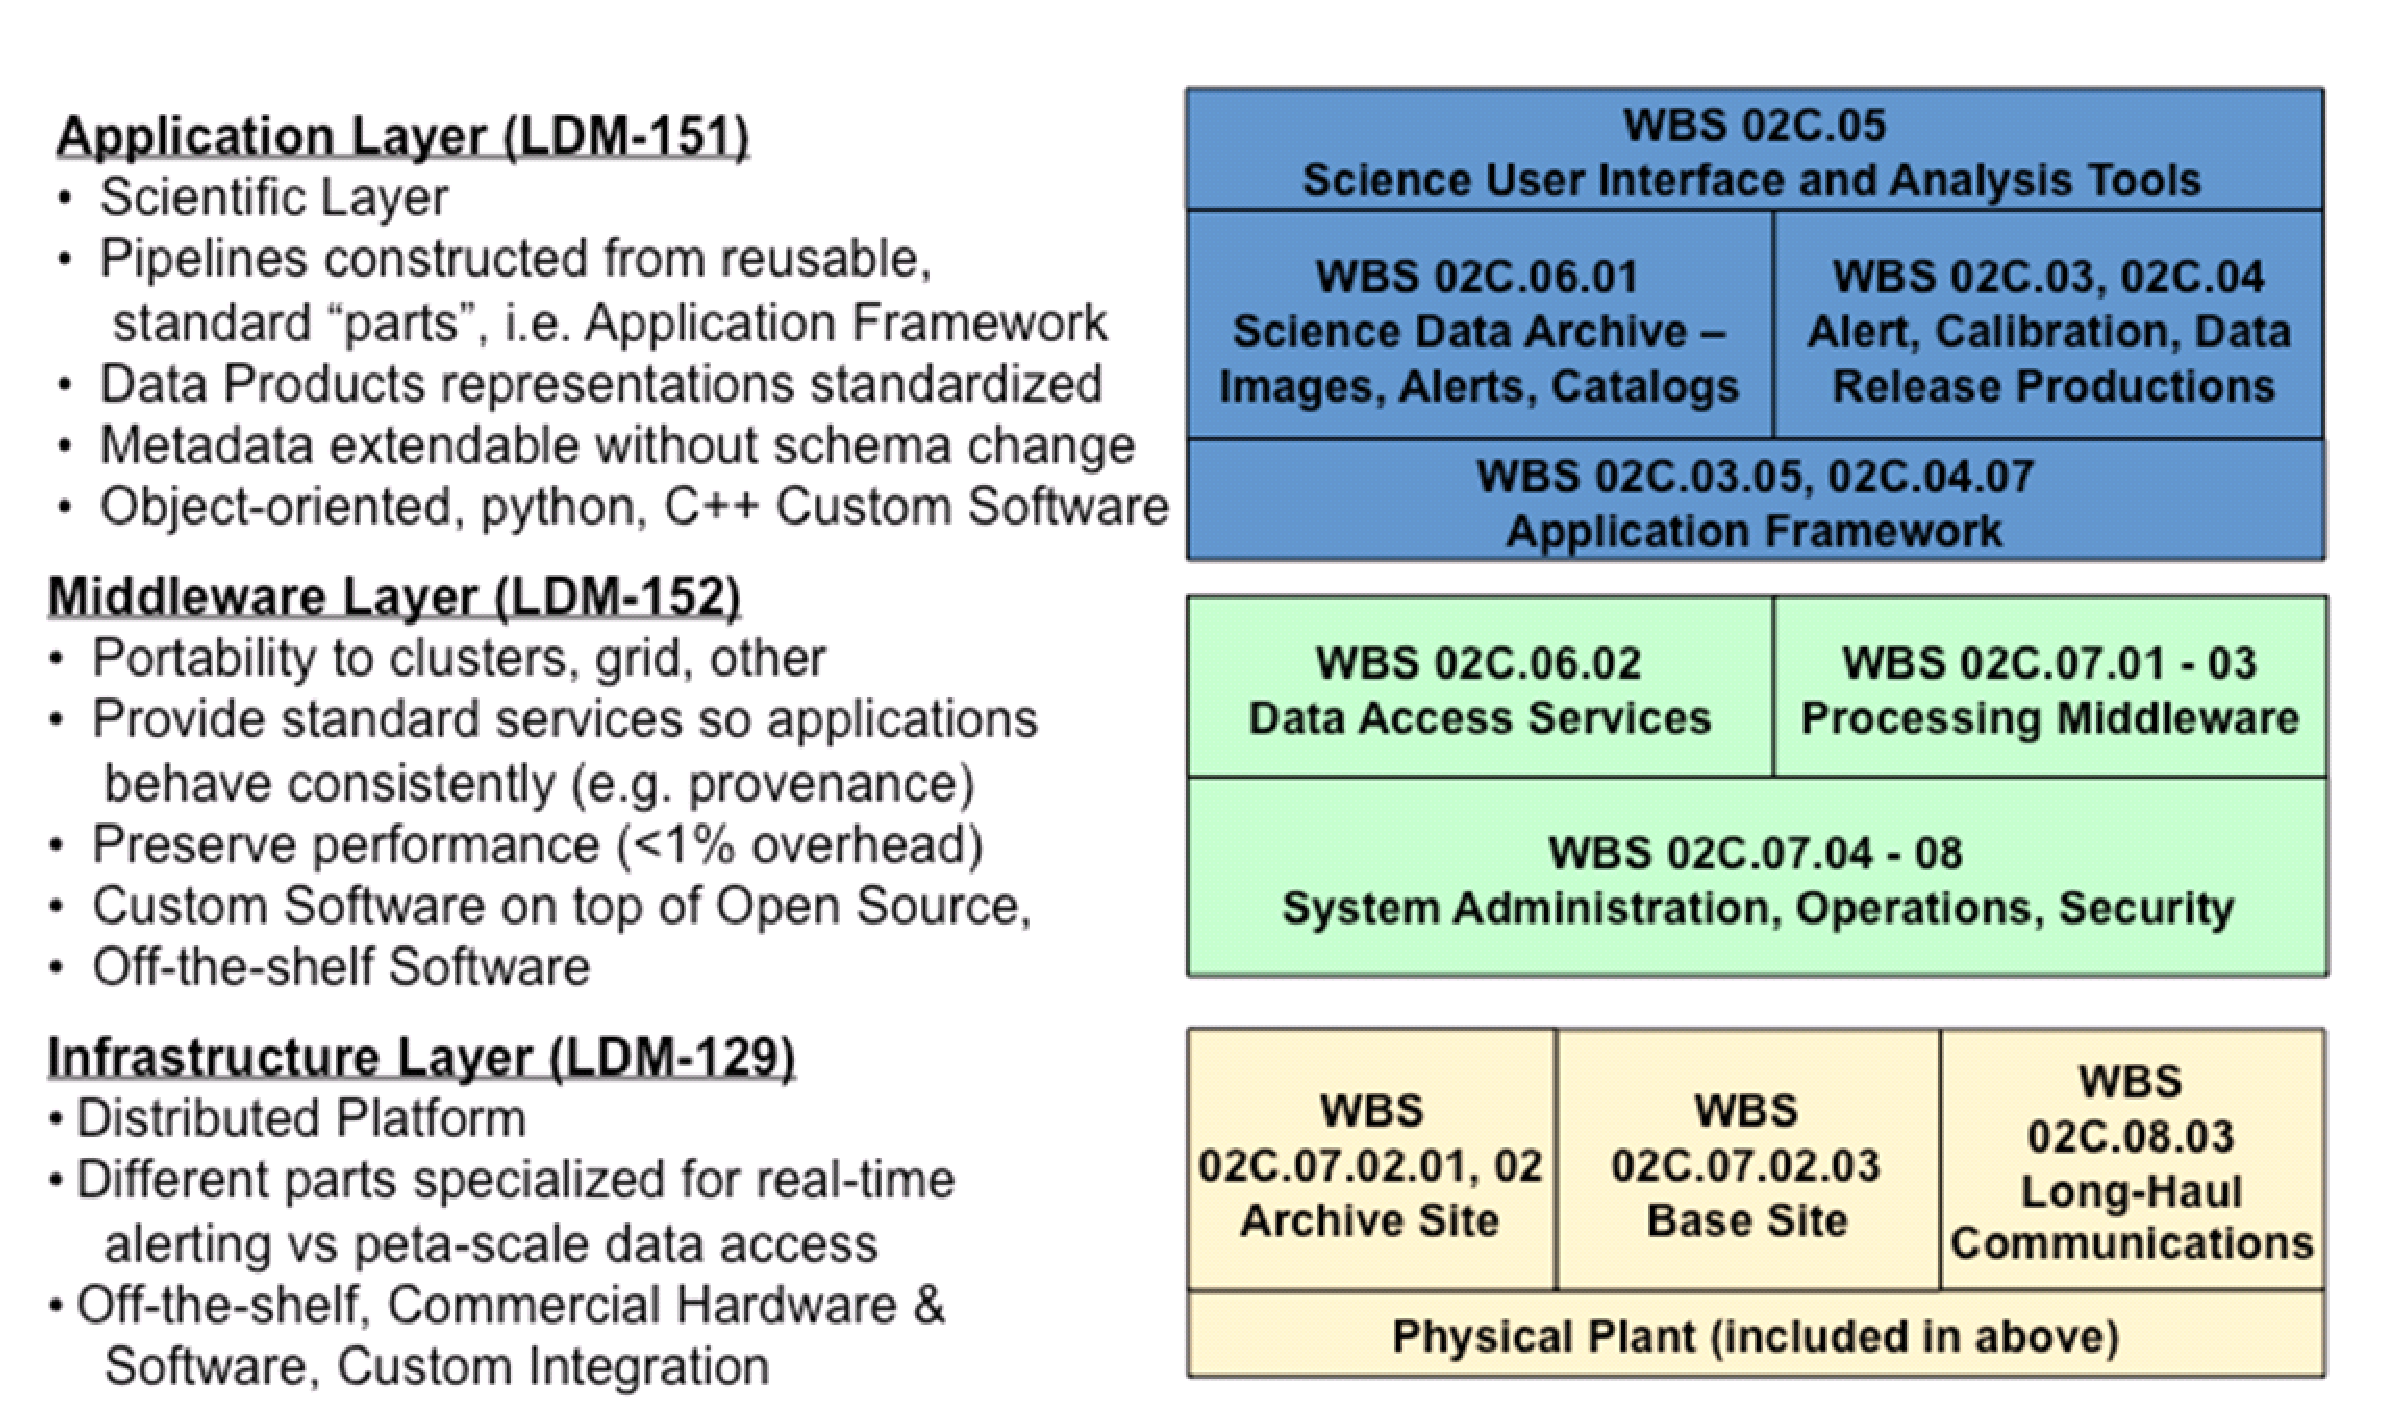
\includegraphics[angle=0,scale=0.40]{LDM148_Fig8.eps}
\caption{Architecture of the Data Management System}
\end{figure}

\begin{figure}
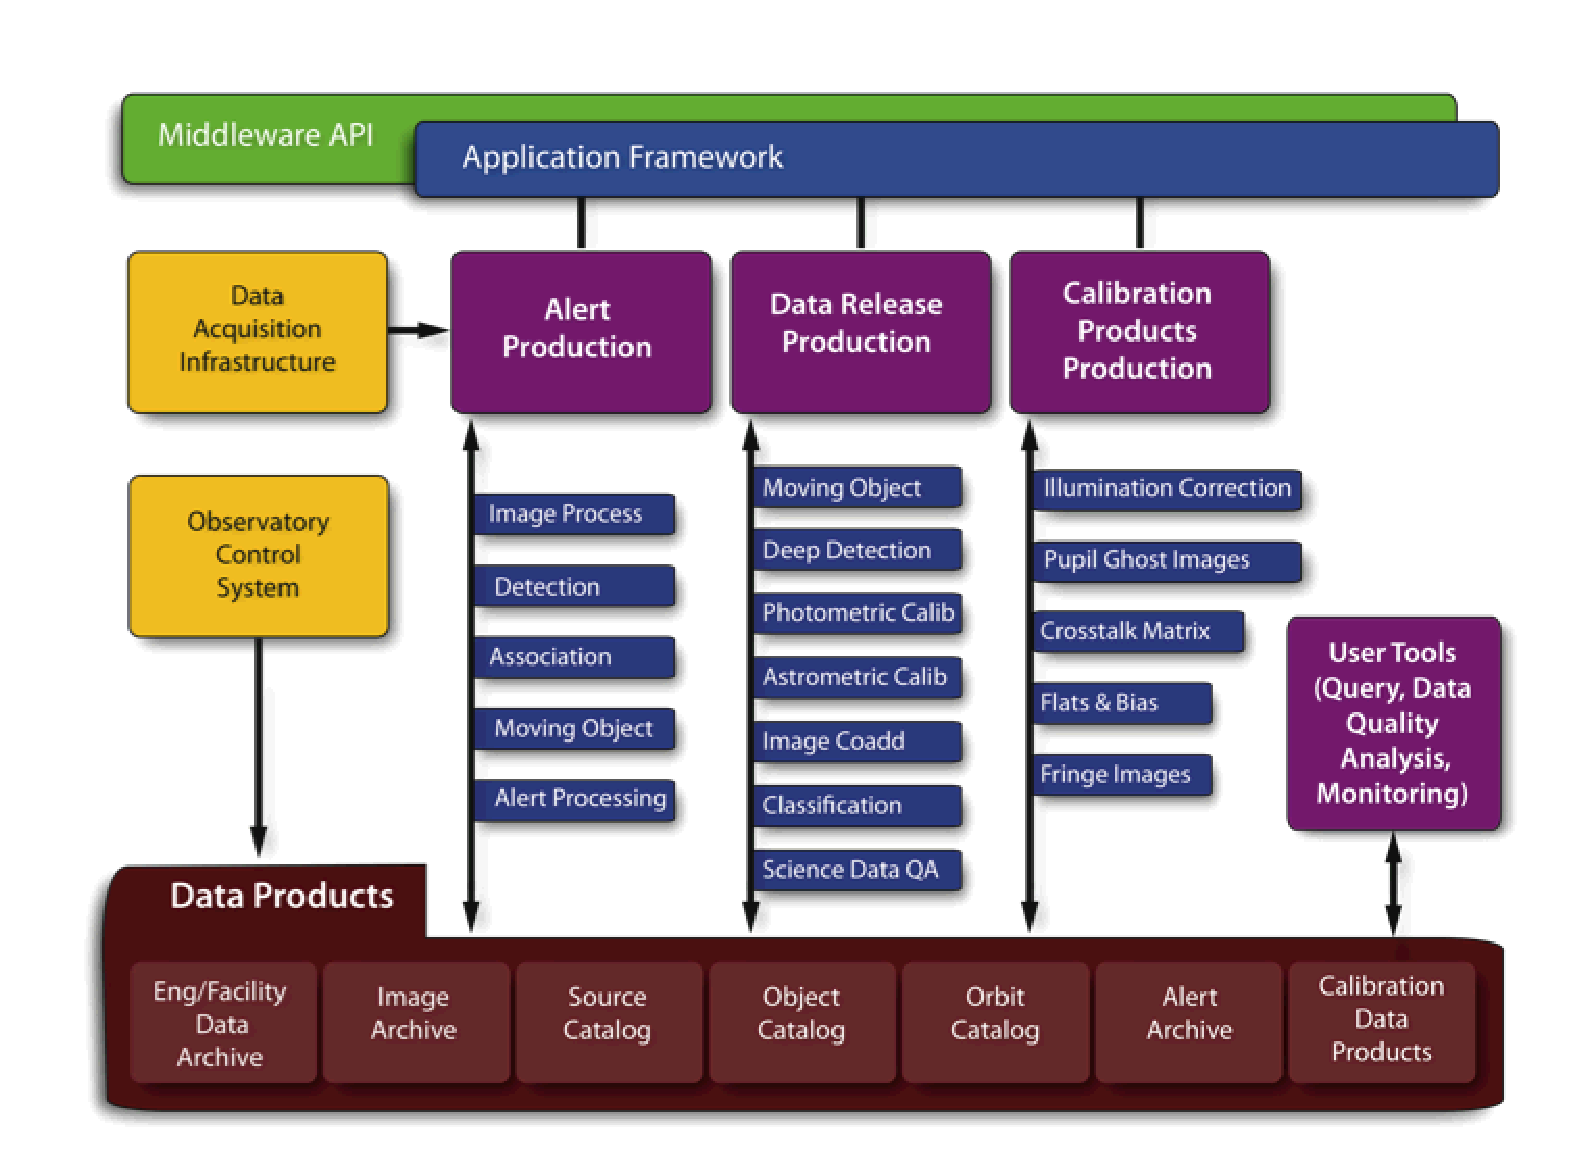
\includegraphics[angle=90,scale=0.70]{ApplicationLayerProductionsandPipelines.eps}
\caption{Organization of DMS Pipelines and Productions}
\end{figure}

\section{LSST Data Product Overview}

\subsection{Level 1, 2, and 3 Data Products}

 The LSST data products are organized into three groups, based largely on
 where and when they are produced.

\begin{itemize}
\item Level 1 products are generated by pipeline processing the stream
  of data from the camera system during normal observing.  Level 1
  data products are therefore continuously generated and / or
  updated every observing night. This process is of necessity highly
  automated, and must proceed with absolutely minimal human
  interaction.  In addition to science data products, a number of
  Level 1 ``SDQA'' data products are generated to assess quality and to provide
  feedback to the Observatory Control System.

\item Level 2 products are generated as part of a Data Release, which
  is required to be performed at least yearly, and will be performed
  more frequently during the first year of the survey.  Level 2
  products use Level
  1 products as input, and include data products for which extensive
  computation is required, often because they combine information from
  many exposures.  Although the steps that generate Level 2 products
  will be automated, significant human interaction may be required at
  key points to ensure the quality of the data.

% where will these humans come from?

\item Level 3 data products are derived from Level 1 and / or Level 2
  data products to support particular science goals, often requiring
  the combination of LSST data across significant areas on the sky.
  The DMS is required to facilitate the creation of Level 3 data
  products, for example by providing suitable ``API''s and computing
  infrastructure, but is not itself required to create any Level 3
  data product. Instead these data products are created externally to
  the DMS, using software written by, eg, science collaborations. Once
  created, Level 3 data products may be associated with Level 1 and
  Level 2 data products through database federation \citep{WikiFedDB}.
  In rare cases, the LSST Project, with the agreement of the Level 3
  creators, may decide to incorporate Level 3 data products into the
  DMS production flow, thereby promoting them to Level 2 data products.

\end{itemize}


Level 1 and Level 2 data products that have passed quality control
tests are required to be accessible to the public without restriction.
Additionally, the source code used to generate them will be made
available, and LSST will provide support for builds on selected
platforms. The access policies for Level 3 data products will be
product- and source-specific, and in some cases will be proprietary.

% Michael's section
\subsection{Overview of Pipeline Processing}
The overall organization of the DMS pipelines and productions is
shown in Fig. 2.  Note that ``production'' in this context has a
particular meaning: it is a coordinated group of pipelines that
together carry out a large-scale DMS function.

\subsubsection{Alert Production - WBS 02C.03}
The Alert Production is directly fed by the output data stream from
the Camera SDS during observing. This data stream contains both
unprocessed (raw) camera images, and images that have been corrected
for crosstalk by the SDS on the mountain.  The normal observing
pattern is to take two 15 second exposures of the same field in immediate
succession.  These two exposures together form a Visit, which is the
data unit processed by the Alert Production.  Its principal
responsibilities are to:

\begin{itemize}
\item Acquire the raw science images from the Camera, and move them to
  the Archive Center for permanent storage.
\item Process the crosstalk-corrected images from the Camera to detect
  transient events within 60 seconds of shutter closure for the second
  exposure in a Visit.
\item Package information about detected transients as
  Alerts, and distribute them to the community as VOEvents.
\item Continuously assess the data quality of the data stream.
\end{itemize}

The major steps in the processing flow, shown in Fig. 3,  are:

\begin{itemize}
\item Image processing of the Raw Exposures to remove the instrumental
  signature. (WBS 02C.03.01)
\item The two images from the Visit (which are termed ``Snaps'') are
  subtracted.  The difference image is scanned for cosmic rays, and
  affected pixels initialize a Mask plane in a new Visit Exposure.  The image
  and variance of the Visit Exposure are summed from the two Snaps.
  These processing steps are encapsulated in the CR Split Handling Pipeline.
  From this point forward, all processing is done with the resulting
  Visit Exposure. (WBS 02C.03.01)
\item Determination of the WCS, PSF, and initial photometric
  zeropoint. This produces Calibrated Science Exposures (Exposures are
  discussed in Section 2.4) (WBS 02C.03.01)
\item Subtraction of a registered and PSF-matched Template Exposure
  from the Calibrated Science
  Exposure, producing a Difference Exposure.  The Template Exposure is
  a coadd created by the Data Release Production (discussed in Section
  4) (WBS 02C.03.07)
\item Detection of sources of either polarity in the Difference
  Exposure, producing DiaSources (discussed in Section 2.3) (WBS 02C.03.01)
\item ForcedDiaSources (Section 2.3), abbreviated measurements of low SNR detections,
  are produced for Objects of particular interest, eg predicted
  positions for Solar System objects, or objects that have previously
  produced Alerts. (WBS 02C.03.01)
\item Comparison of positive flux DiaSources with predictions from
  NightMOPS, the Alert Production component of the Moving Object
  System (MOPS), for already known Solar System objects, as contained in the
  MovingObject table (Section 2.3) (WBS 02C.03.06)
\item The Association Pipeline is run to match DiaSources to already
  known astronomical objects, as contained in the Object table
  (Section 2.3) (WBS 02C.03.02)
\item Generation of Alerts.  DiaSources that are not matched to a known Solar System
  object,  will produce an Alert (Section 2.4) (WBS 02C.03.03)
\item SDQA is performed at every pipeline stage, stored in database
  tables, and fed to the OCS as required. (WBS 02C.01.02.01)
\item DayMOPS, the track detection and orbit fitting component of
  MOPS, is run during the day to interpret each new detection of a
  moving object as a new measurement of a Solar System object already
  in the MovingObject table, or as a previously unknown object, which
  will be added to the MovingObject table.  All orbits are refined
  based on the new measurements from the night. (WBS 02C.03.06)
\end{itemize}

As the raw images arrive at the Archive Center, the same processing
flow is performed there, with the consistency of the databases at the
Base and Archive Centers being periodically checked.  The duplication
of processing is carried out to reduce the data bandwidth required
between the Base and Archive Centers.

\subsubsection{Alert Production Prototypes}
Most components of the Alert Production have been prototyped in the
Data Challenges.  In most cases, algorithmic functionality is close to
LSST requirements, but with data flows at greatly reduced scale. The
prototype status is as follows:
\begin{itemize}
\item WBS 02C.03.01:  Has been completely prototyped, with the
  exception of the CR Split Handline Pipeline, which has been
  partially prototyped.
\item WBS 02C.03.02: Completely prototyped
\item WBS 02C.03.03: Not prototyped
\item WBS 02C.03.06: Prototyped and functional, but outside of DMS software framework
\item WBS 02C.03.07: Completely prototyped
\end{itemize}

\begin{figure}
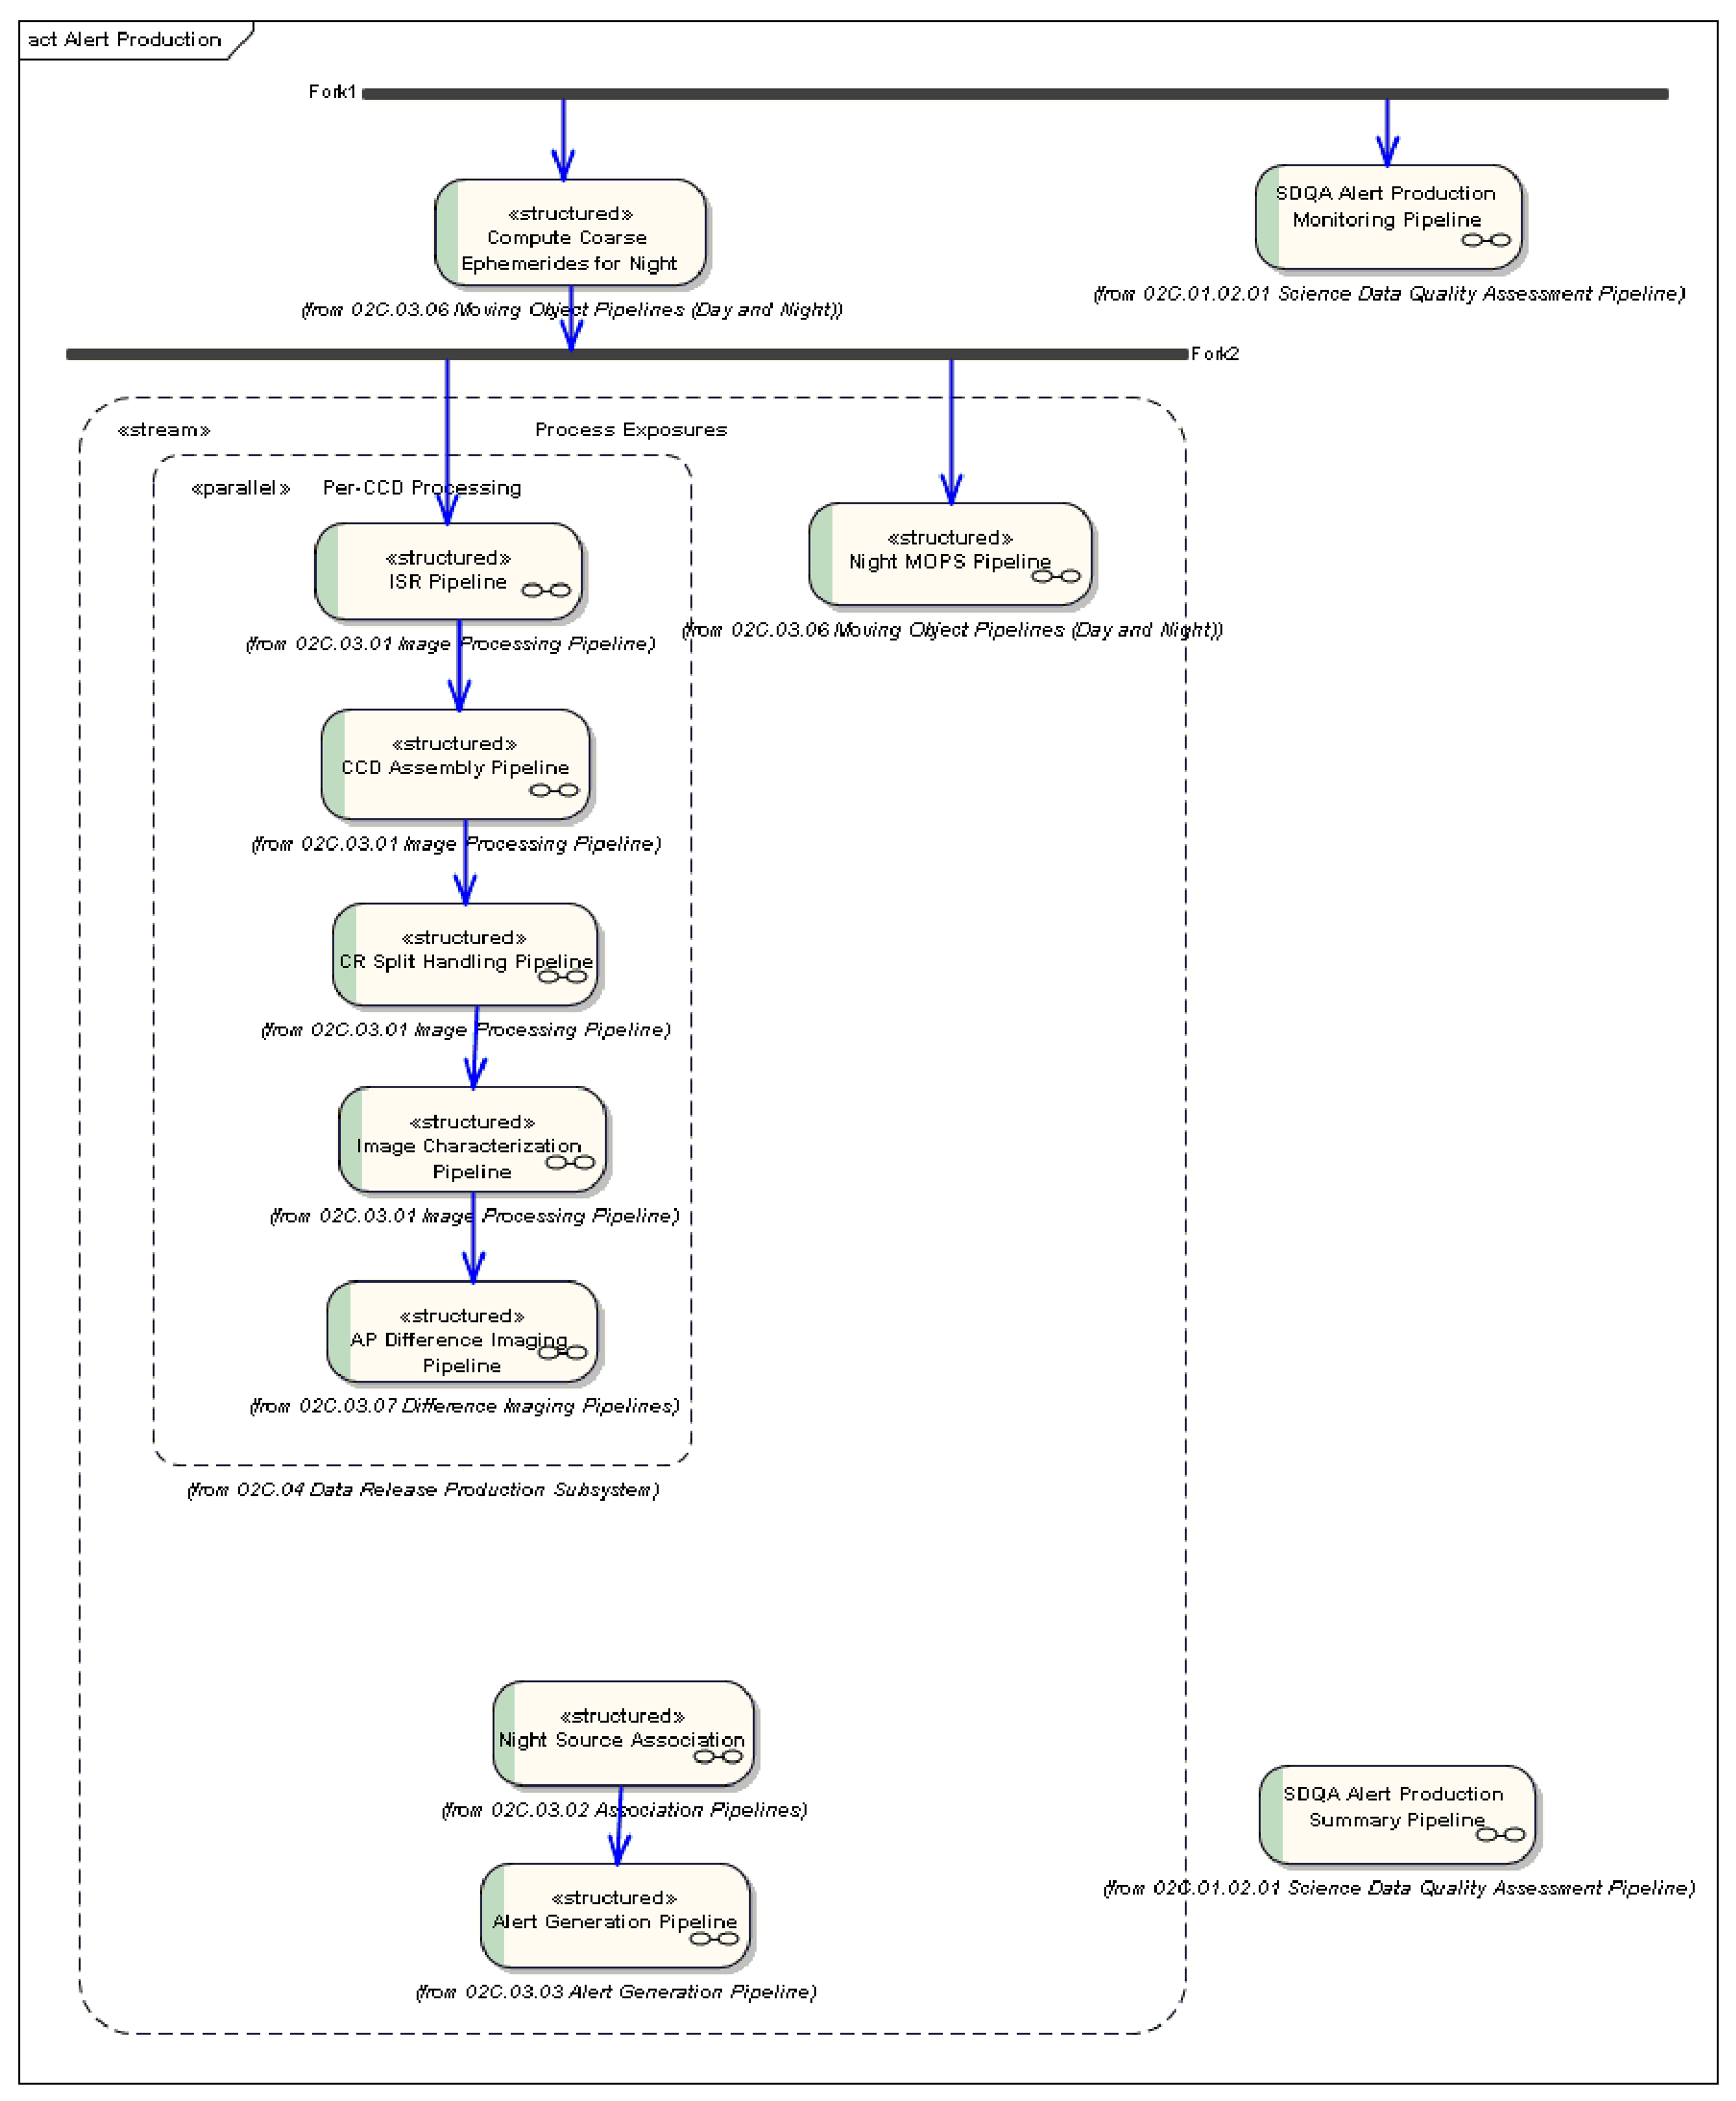
\includegraphics[angle=0,scale=0.40]{AlertProduction.eps}
\caption{Alert Production Processing Flow}
\end{figure}

\subsubsection{Data Release Production - WBS 02C.04 }
At yearly intervals (more often during the first year of the survey) a
new Data Release is produced.  A DR includes all data taken by the
survey from day one to the cutoff date for the DR, and is a
self-contained set of data products, all produced with the same
pipeline software and processing parameters.  The major steps in the
processing flow, shown in Fig. 4,  are:

\begin{itemize}
\item As in the Alert Production, all Raw Exposures from the camera
  are processed to remove the instrumental signature, and to determine
  the WCS and PSF, producing Calibrated Science Exposures.  This is done with
  the best available calibration products, which in general will not
  be those available when the processing was initially done.  Unlike
  the Alert Production, which uses images corrected for crosstalk by
  the Camera System, the Data Release Production will do its own
  crosstalk production, since the crosstalk correction matrix may be
  updated since the image was collected. (WBS 02C.03.01)
\item The Astrometric Calibration Pipeline is run on the full set of
  measurements in the Source catalog.  This generates astrometric
  models, including proper motion, parallax, and possibly binary
  parameters, for all Objects which are bright enough to be above the
  single Exposure detection limit.  Additionally, the relative astrometric
  calibration of each ccd is known at all pixel positions to a few
  milli-arcsec, making the subsequent production of coadds more
  accurate. (WBS 02C.04.02)
\item The survey region is tessellated into a set of sky patches, and
  several Coadded Exposures are produced for each patch from the
  Calibrated Science Exposures.  These are a per-band Template Coadd used for image
  subtraction; a Detection Coadd used in the Deep Detection Pipeline,
  possibly per-band; and a RGB Coadd used for visualization. (WBS 02C.04.04)
\item The Deep Detection and Object Characterization Pipelines are run (see Section 6), populating the
  Object, Source, and ForcedSource tables.  Object Characterization uses a
  combination of the
  stackfit and multifit algorithm (discussed in Section 6.2) to fit object
  models to the entire stack of Exposures which contain
  the Object. This results in a set of measurements of the Object
  attributes over the full time span of the survey, including
  astrometric parameters such as proper motion and parallax. (WBS
  02C.04.05, 02C.04.06)
\item The Image Subtraction Pipeline is run, as in the Alert
  Production, yielding DiaSources and ForcedSources (see Section 6),
  for transient objects (WBS 02C.03.07)
\item The Moving Object Pipeline is run on DiaSources, to yield a
  complete set of orbits for Solar System Objects in the MovingObject
  table. (WBS 02C.03.06)
\item The Photometric Calibration Pipeline is run on the full set of
  measurements in the Source, DiaSource, and ForcedSource catalogs,
  incorporating measurements from the Calibration Telescope and other
  sources of data about the atmosphere to perform a global photometric
  calibration of the survey.  In addition to accurate photometry for
  every measurement, this yields an atmosphere model for every
  Exposure. (WBS 02C.04.01)

\end{itemize}

\subsubsection{Data Release Production Prototypes}
About 50\% of the components of the Data Release Production have been prototyped in the
Data Challenges.  The
prototype status is as follows:
\begin{itemize}
\item WBS 02C.03.01: As for Alert Production
\item WBS 02C.03.02: Completely prototyped
\item WBS 02C.03.03: Not yet prototyped
\item WBS 02C.03.06: Prototyped and functional, but outside of DMS software framework
\item WBS 02C.03.07: As for Alert Production
\item WBS 02C.04.02: Prototyped and functional, but outside of DMS
  software framework
\item WBS 02C.04.01: Set up and solution of self calibration system
  has been prototyped outside of DMS software framework
\item WBS 02C.04.03: Prototyped, but galaxy model measurements not yet
  to LSST requirements
\item WBS 02C.04.04: Detection coadd prototyped.
\item WBS 02C.04.05: Not yet prototyped
\item WBS 02C.04.06: Not yet prototyped

\end{itemize}

\begin{figure}
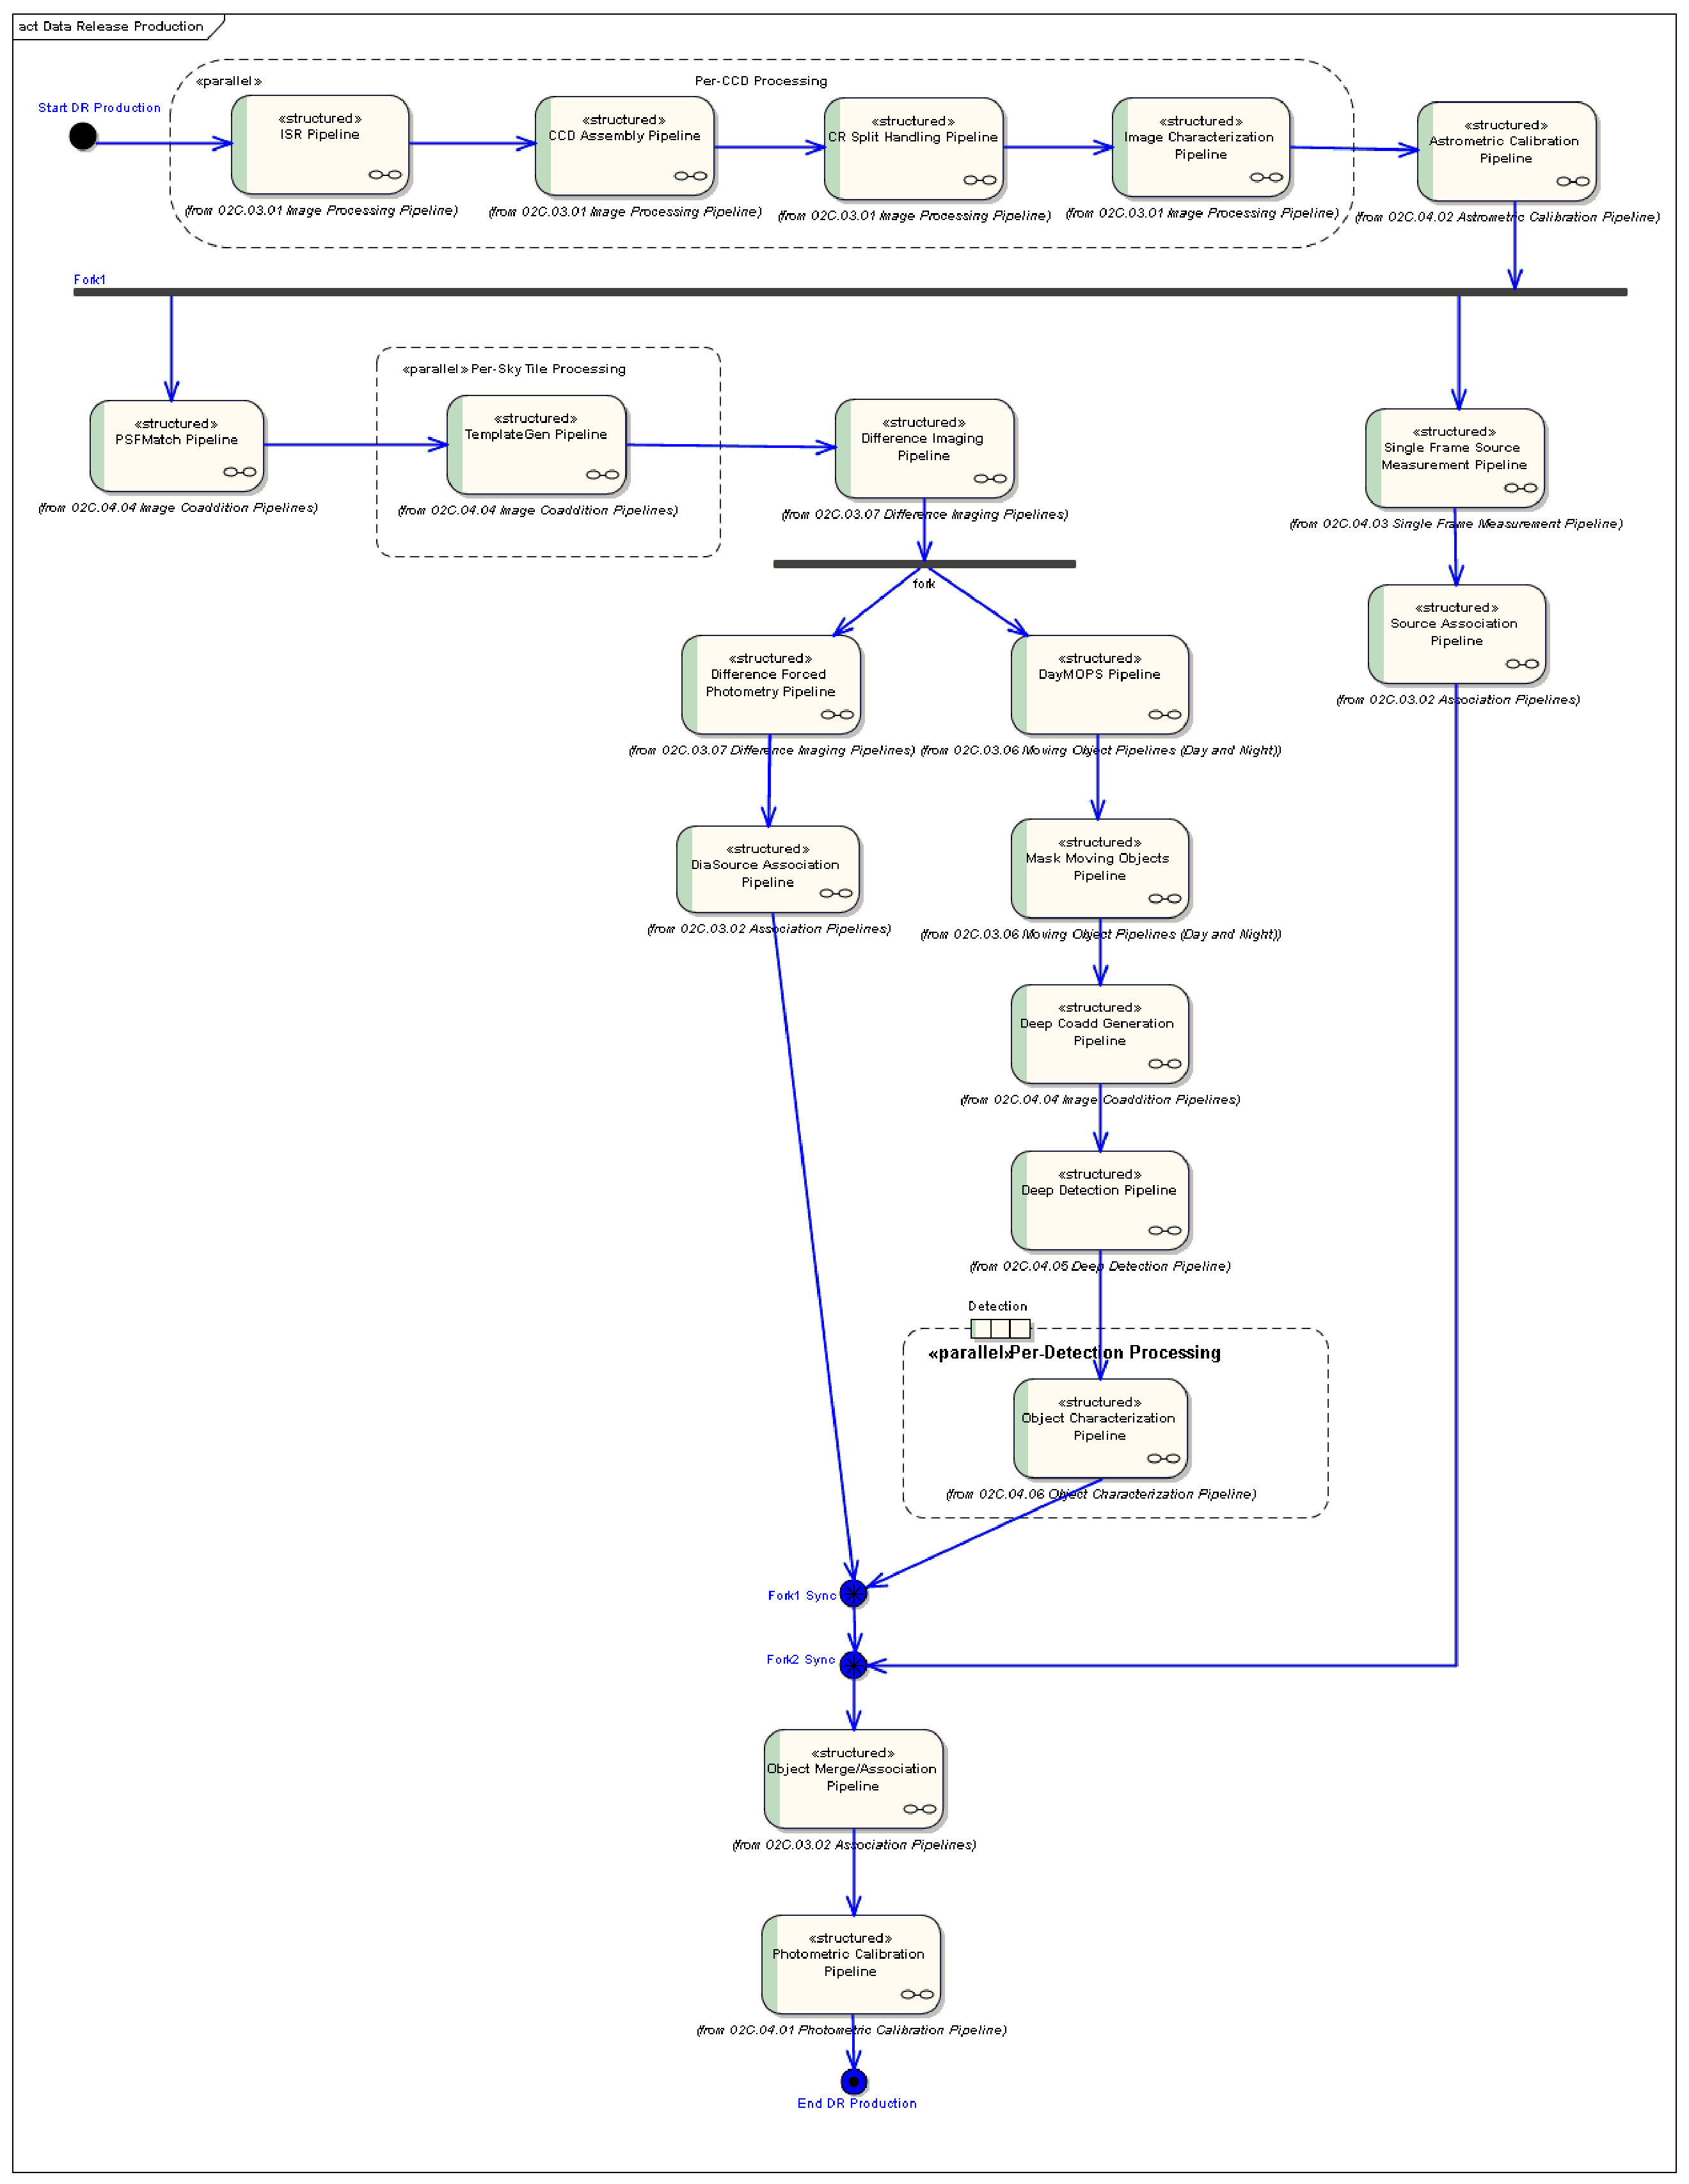
\includegraphics[angle=0,scale=0.40]{DataReleaseProduction.eps}
\caption{Data Release Production Processing Flow}
\end{figure}

\subsubsection{Calibration Products Production - WBS 02C.03}
A variety of calibration products are required by both the Alert
Production and Data Release Production.  The Calibration Products
Production is run as required (intervals TBD, dependent on experience with
system stability) to produce them, as listed in Section 4.  As shown
in Fig. 5, the
activities contained within the Calibration Products Production are:

\begin{itemize}
\item Produce Master Dark Current Exposure 
\item Produce Master Flat Exposure 
\item Produce Atmospheric Models from Calibration Telescope Spectra
\item Produce Pupil Ghost Exposure
\item Produce Crosstalk Matrix
\item Produce Master Bias Exposure
\item Produce Illumination Correction Exposure
\item Produce Master Fringe Exposure
\end{itemize}

\subsubsection {Calibration Products Production Prototypes}
The Calibration Products Production has not yet been prototyped.
Calibration products needed for testing the Alert Production and Data
Release Production have been generated by hand with the usual
astronomical tools.

\begin{figure}
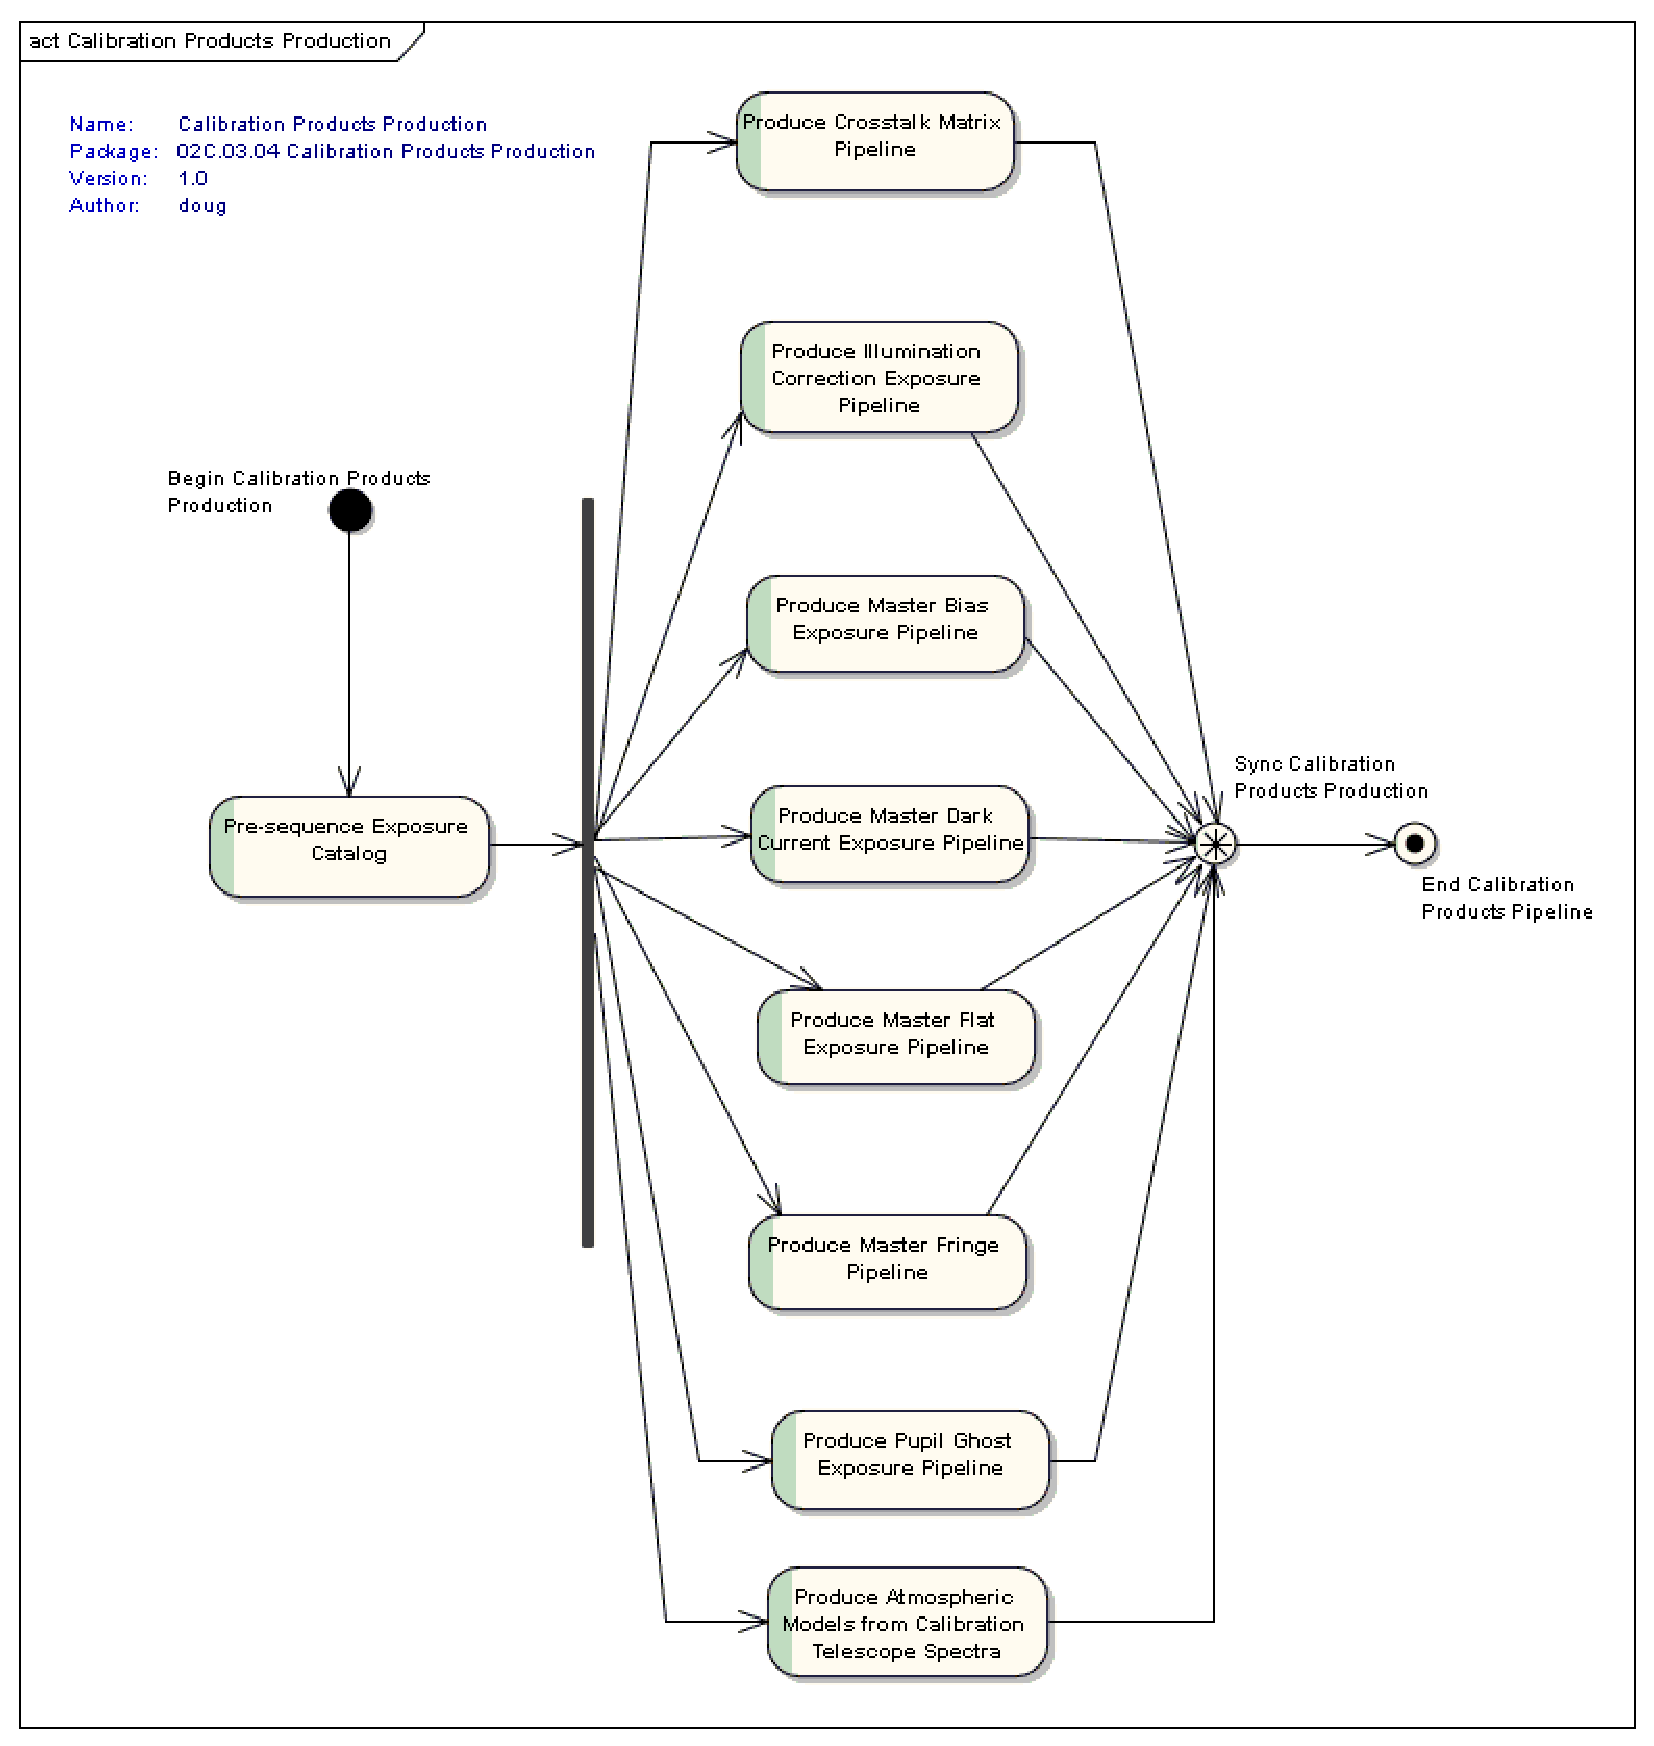
\includegraphics[angle=0,scale=0.40]{CalibrationProductsProduction.eps}
\caption{Calibration Products Production Processing Flow}
\end{figure}

\subsection{Contents of Principal Database Tables}

All catalog data is stored in tables within a relational
database, the ``Science Database''.  The current Science Database
schema, which continues to evolve, is always available at \newline
\verb+http://dev.lsstcorp.org/schema/+. This narrative does not
explain this schema in detail, but instead focuses on the contents of
a few key tables and the logic by which that content is generated.

Two important definitions that underly the design of the database are
those for ``Object'' and ``Source''.  An ``Object'' (or, when confusion is
possible, an ``AstroObject'') is a representation of an astrophysical
object:  a star; a galaxy; a Solar System object.   A ``Source'' is the
representation of a measurement of an Object's properties from a
single image that contains its footprint on the sky.  As we discuss in the
remainder of this section, both Objects and Sources come in a few
different flavors that are specialized for particular situations that
frequently arise.

The relationships of the central tables of the Science Database are
shown in Fig. 6.  The highest level tables are Object and
MovingObject, which together organize on a per-astrophysical-object
basis all information from the survey.  An entry in either of these
tables links to all the individual measurements of the Object,
contained in the DiaSource, ForcedSource, and Source tables.  Each of
these measurements, in turn, links to the metadata for each telescope
exposure in the Exposure table.

\paragraph{Object Table}

% Rob wants a definition of ``found'' - means coadd + DIA; ZI scheme
% goes here
% Note that an Object can changes tables
The Object Table has a row for every non-Solar-System astrophysical
object found in the LSST images.  Each Object Table row has a set of
columns which together summarize what has been measured for the object
over the history of the survey.  The information falls into two
categories:

\begin{itemize}
\item Band-independent information
\begin{itemize}
\item Object identification and naming information
\item Bounding box on sky
\item Astrometric parameters - mean position, proper motion, parallax
\item Photometric redshift
\item Extendedness probability
\item Variability probability
\item Data quality flags
\end{itemize}
\item Per-band information
\begin{itemize}
\item Model parameters and covariances for each model fit to the Object (see Section 6.2.3)
\item Light curve summary parameters
\item Photometric redshift
\item Data quality flags
\end{itemize}
\end{itemize}

% can first two digits of Id = DR# for human readability?
\paragraph{MovingObject Table}

% ref PS-MOPS?
Solar system objects are detected in difference images as DiaSources
with positive flux.  These sources are then processed by the Moving
Object Pipeline (MOPS), which links sources together into tracks of
individual objects and determines orbits for them.  The LSST MOPS is
derived from PanSTARRS MOPS \citep{MOPS} The information includes:

\begin{itemize}
\item MovingObject identification
\item Orbital elements
\item Average photometric properties in each band
\item Data quality flags
\end{itemize}

Note that there will be occasions during nightly alert processing in
which an Object with only a single associated measurement is
subsequently found to be a measurement of a MovingObject.  In these
relatively rare cases, the original Object will be deleted.
% -----------------------------------------------------------------------------------------------------------------
\paragraph{Source Table}

An entry in the Source Table is made in conjunction with Single
Exposure Measurement of an Object.  These measurements have relatively
high signal-to-noise, and include the following information:

\begin{itemize}
\item Source identification
\item Associated Object identification
\item Set of position measurements and their covariances
\item Set of flux measurements and their variances
\item Set of shape measurements and their variances
\item Sky level and its variance
\item Photometric calibration corrections
\item Data quality flags
\end{itemize}

\paragraph{DiaSource Table}
An entry in the DiaSource Table is made as a result of a high SNR
measurement of an Object in a difference Exposure. The information
contained in the DiaSource Table is a simplified form of the Source
table quantities.

\paragraph{ForcedSource Table}
An entry in the ForcedSource Table is made in conjunction with a low
SNR measurement of an Object either with Multifit or in a difference
Exposure. The information contained in the ForcedSource Table is:

\begin{itemize}
\item ForcedSource identification
\item Associated Object or MovingObject identification
\item Pixel coordinates where the flux was measured
\item Measured flux and its variance
\item Data quality flags
\end{itemize}

\paragraph{Exposure Table}
The Exposure Table contains the most frequently needed metadata for an
Exposure.  Additional metadata can be obtained from the Engineering
and Facility Database, which can be queried together with the Science
Database. The information contained in the Exposure Table includes:
\begin{itemize}
\item Exposure identification
\item Time of Exposure midpoint
\item Exposure time
\item Filter Id
\item WCS
\item Camera metadata
\item Telescope metadata
\end{itemize}


% -----------------------------------------------------------------------------------------------------------------
\begin{figure}
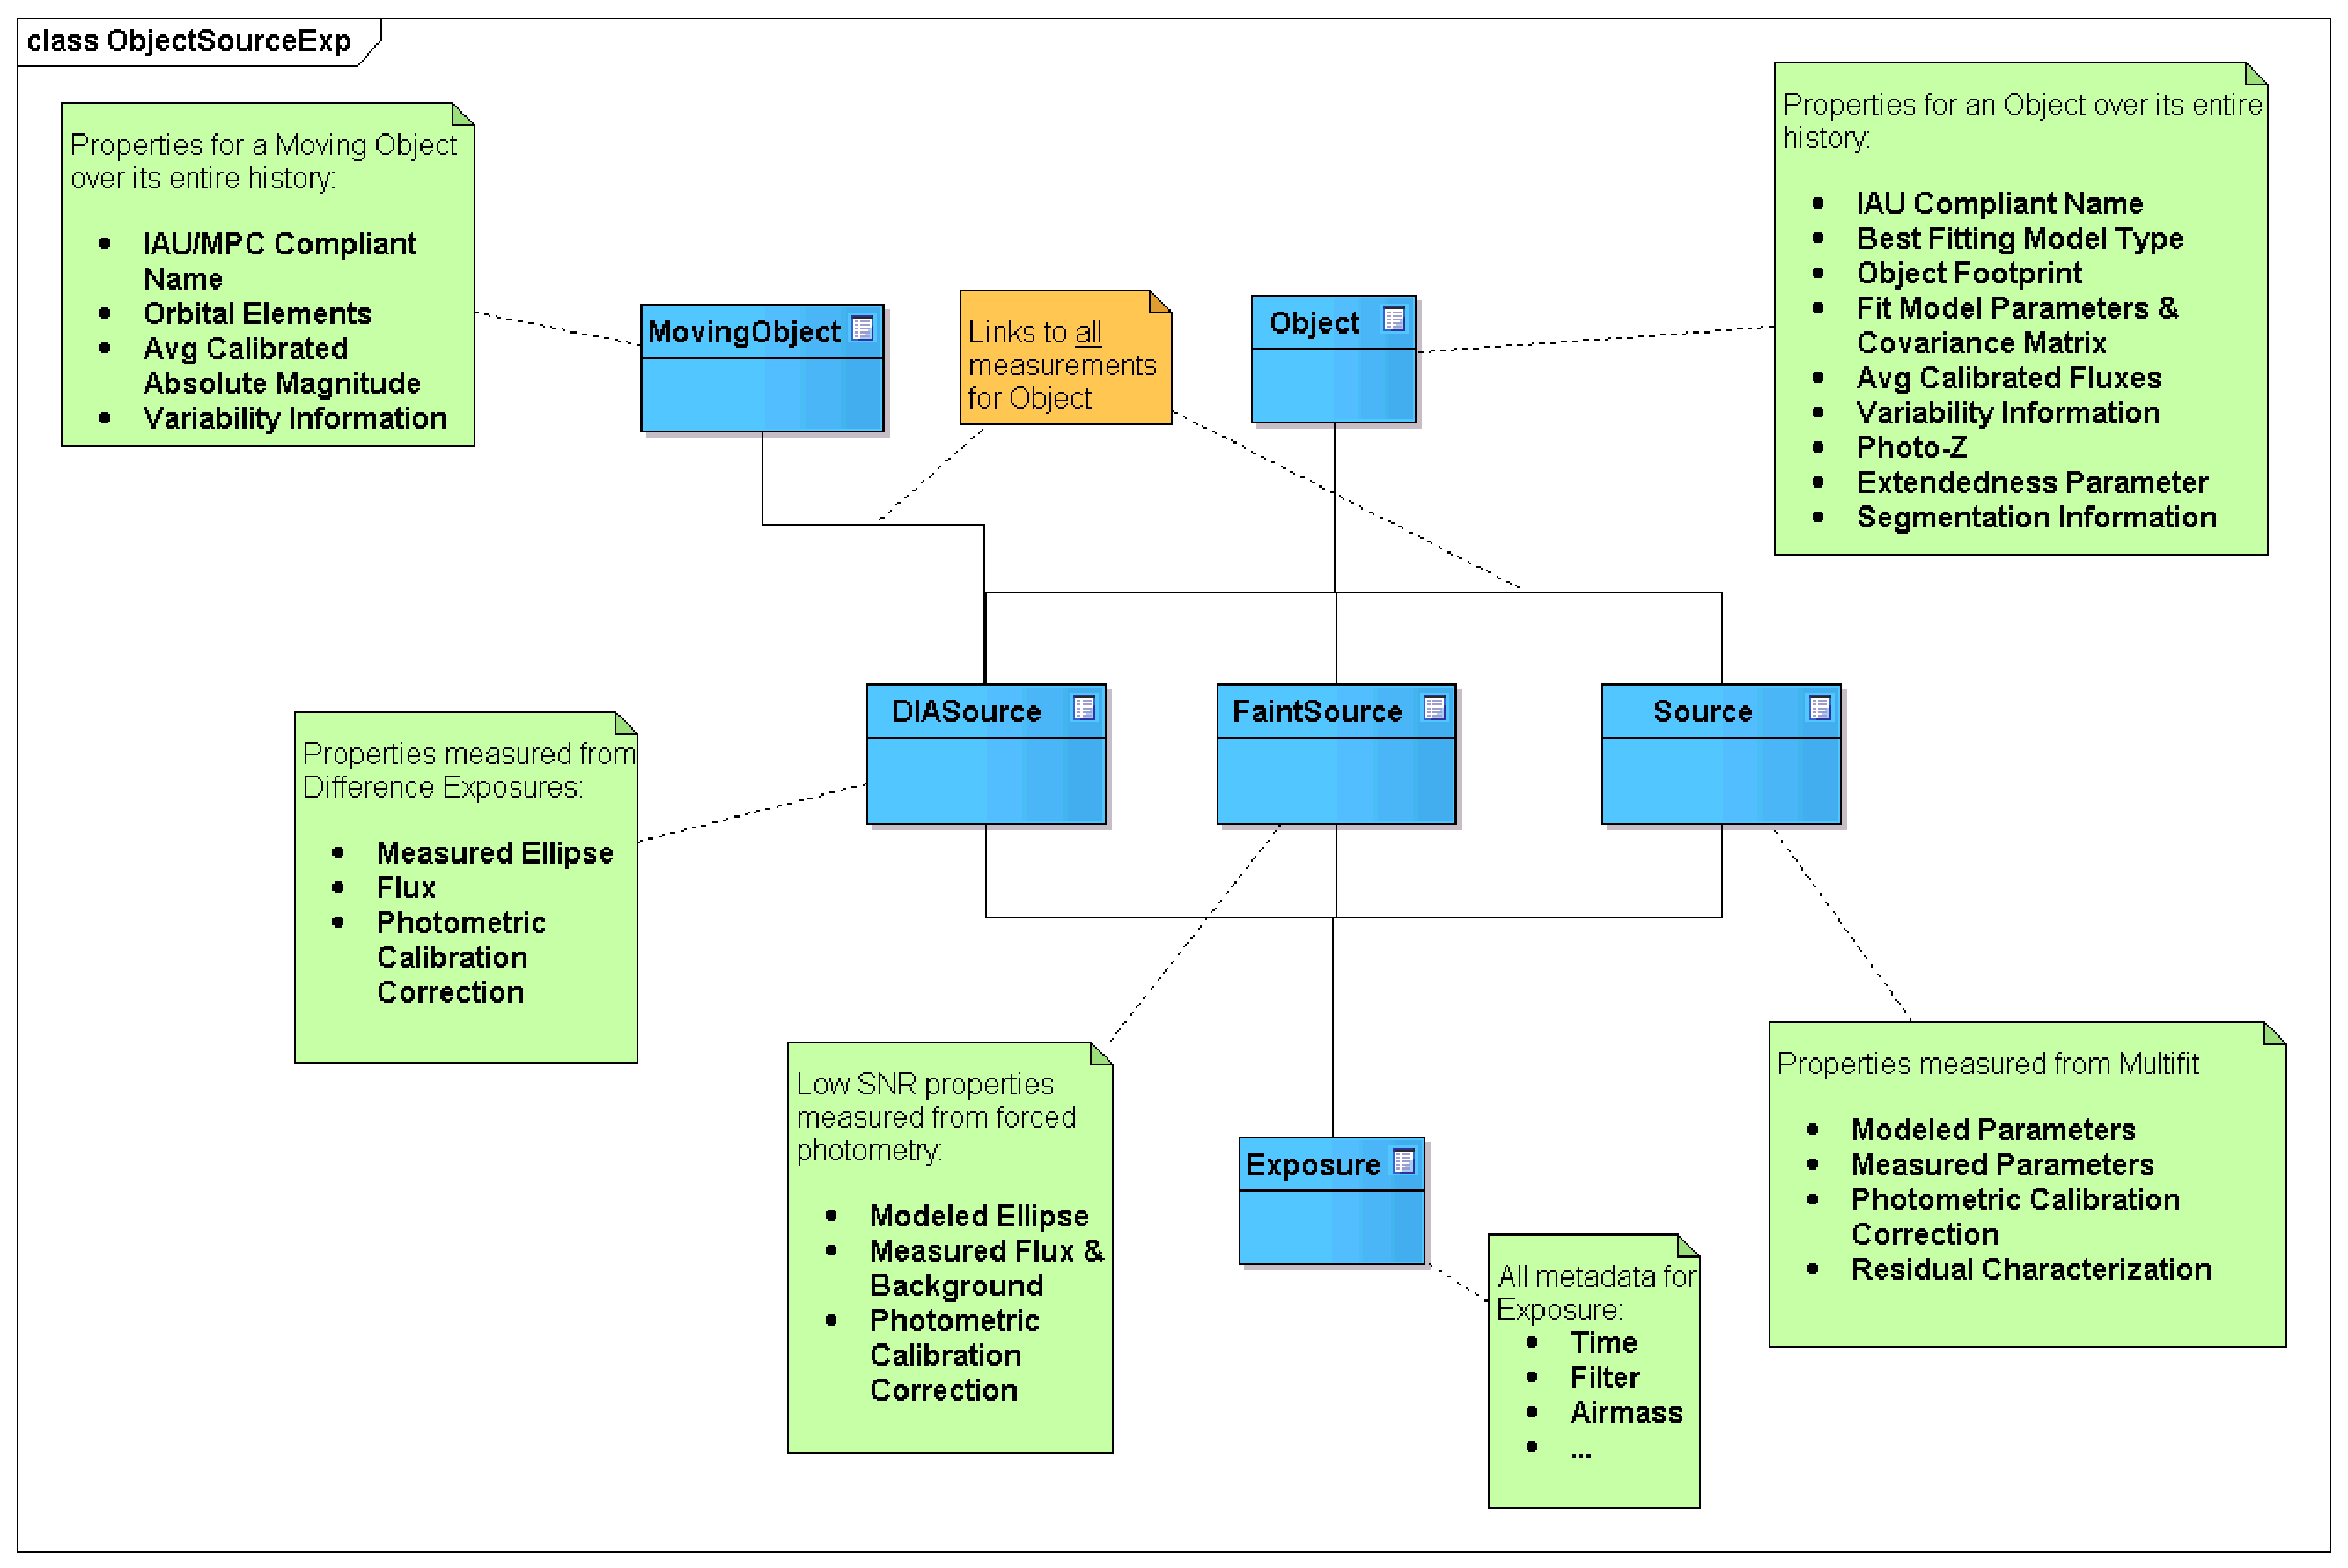
\includegraphics[angle=90,scale=0.50]{ObjectSourceExp.eps}
\caption{Key tables in the LSST database schema}
\end{figure}

\subsection{Common Data Objects}
Level 1 and 2 data products are both built from common data objects that
are also used throughout the pipeline systems.  These may be utilized for
Level 3 data products as well.  This is the list of the top level data objects:

\paragraph{MaskedImages}
A ``MaskedImage'' contains pixel data.
A MaskedImage may cover a whole focal plane, a
single CCD, or a CCD segment. The pixel data, which is all on the same
grid, consists of:
\begin{itemize}
\item the Science image, with the pixel data type being either 16-bit
  integers or 32-bit floats.
\item the Mask image, typically 16 bits deep, with each plane representing
  a particular logical statement about the corresponding science image pixel, eg ``this pixel is
  saturated''.
\item the Variance image, which represents the expected variance in the
  corresponding science pixel values
\end{itemize}

\paragraph{Exposures}
An ``Exposure'' is a MaskedImage associated with a variety
of image metadata.  The types of image metadata contained in an
Exposure depends on the processing steps applied to the Exposure, so
that a Raw Exposure will have relatively basic metadata that comes
directly from the OCS, while a Calibrated Science Exposure may have in addition
a WCS, a PSF, and a model of atmospheric transmission as a function of
field position.

\paragraph{Coadded Exposures}
A Coadded Exposure results from combining multiple overlapping
Exposures, potentially from multiple filters. In the combination
process, the images are reprojected to a common coordinate system.
The pixel data has the same components as a MaskedImage.  The image
metadata differs, however, and will be stored in its own table (still
TBD).

\paragraph{Alerts}
An Alert is a notification to the community that a transient event has
been observed by the LSST. The community has strongly expressed the
preference that Alerts not be significantly filtered prior to
distribution so that science opportunities are not closed off.  We
have therefore adopted very simple criteria for issuing an Alert: A
5-sigma (operational choice TBD) DiaSource was seen in both
Exposures of a Visit which are not consistent with cosmic ray
events. 

The data bundled with the Alert includes:
\begin{itemize}
\item The rows from the Exposure table for the two Exposures in the
  Visit
\item The rows from the DiaSource table for the two relevant
  DiaSources
\item The row from the Object table for the associated Object.
\item A postage stamp image centered on the DiaSource from each of the
  two Difference Exposures, and from the Template Exposure
\end{itemize}

Note that no explicit classification of an Alert is provided, but
users can readily construct classifiers and filters based on information in the
Science Database.  This includes past time dependence, colors, and
shape information for the associated Object.  Additionally, database
queries can readily be formulated which will identify Exposures that
have generated anomalously large numbers of Alerts, presumably due to
image artifacts or processing problems.

\section{Level 1 Data Products}

\paragraph{Exposures}
The following Level 1 Exposures will be available
\begin{itemize}
\item Raw Exposures
\item Calibrated Science Exposures (trimmed, debiased, flattened, etc)
\item Difference Exposures
\end{itemize}
Note that the Raw Exposures are sent to the
Archive Center, where they are immediately made available for
retrieval.  Calibrated Science and Difference Exposures are recreated on-the-fly
at the Archive Center as needed.
\paragraph{Catalogs}
The following catalogs are updated through the nightly running of the
Alert production.  With the exception of Exposure, they are all
recreated from scratch during the production of each Data Release.
\begin{itemize}
\item Exposure
\item Object
\item MovingObject
\item DiaSource
\item ForcedSource
\end{itemize}
\paragraph{Alerts}
Alerts are distributed as VOEvents, and archived at the Archive Center

\paragraph{Nightly Summary Products}
A variety of reports will be generated every night to summarize the
performance of the DMS and the SDQA metrics on the Level 1 data. The
contents of these is TBD.
\paragraph{Engineering and Facility Database Archive}
Every 24hrs, the DMS synchronizes the Engineering and Facility
Database, which is generated by the Observatory Control System (OCS),
with the copy at the Archive Center. This Level 1 product contains
comprehensive metadata for the entire LSST observatory, and can be
queried together with the Science Database.
\section{Level 2 Data Products}
\paragraph{Coadded Exposures}
The following Coadded Exposures are Level 2 Data products
\begin{itemize}
\item Template Coadd for creating Difference Exposures.   This Coadd
  is optimized for a narrow PSF, so that during image differencing the
  Template is never narrowed by the matching kernel, even in the best seeing of the
  survey. A Template is specific to a filter band.
\item Detection Coadd for object detection.  This Coadd is optimized
  so that the peaks from faint objects have the highest
  signal-to-noise. The Detection Coadd may combine information from
  multiple filter bands.
\item RGB Coadd for visualization.  This Coadd will be formed by
  combining the Template Coadds for the individual filter bands to
  give a visually pleasing and useful color image.
\end{itemize}
\paragraph{Calibration Products}
The Calibration Products Production generates the full range
of calibration products necessary for the functioning of the Alert and
Data Release Productions.  The products include, on a
per-filter basis when required:
\begin{itemize}
\item Bias Exposures
\item Monochromatic Dome Flats
\item Broadband Dome Flats
\item Pupil Ghost Image
\item Crosstalk Correction Matrix
\item Fringe Images
\item Illumination Correction
\item A variety of products required for the Calibration Telescope (TBD) 
\end{itemize}
\paragraph{Catalogs}
With the exception of Exposure, the following catalogs are created
from scratch during the production of each Data Release. Exposure is
updated with the latest derived metadata, such as WCS and PSF.
\begin{itemize}
\item Exposure
\item Object
\item MovingObject
\item Source
\item DiaSource
\item ForcedSource
\end{itemize}

\section{Level 3 Data Products}
Level 3 data products are derived from Level 1 and
Level 2 data products, usually requiring the use of LSST data across
significant areas on the sky.  These may be the results of large
queries, or derived catalogs which require pixel-level reprocessing of
some quantity of image data.  Examples include:

\begin{itemize}
\item phase-folded light curves for periodic variables
\item catalogs of specific subsets of objects
\item maps of derived properties such as lensing shear
\item catalogs of clusters
\item catalogs of morphologically analyzed galaxies
\end{itemize}

An essential feature of Level 3 data products is that their creation
is not a responsibility of the DMS.  They will arise from user
analysis projects. �The generation of Level 3 data products may thus
involve the use of code and query definitions from outside the LSST
project, and that is not part of the project's open-source code base.
When Level 3 data products are created as the output of analysis of 
LSST data, whether with the basic interactive user tools or via
custom pipelines, tools will be provided so that they may be federated
with the Level 1 and Level 2 datasets, so that 
joins may easily be made between data-release and user-provided tables.

It is anticipated that certain of the Level 3 data products will be
archived by the DMS, using project resources provided for this
purpose.  The allocation of these resources to archiving, and the
duration of storage, will be determined by the LSST Project based on
the value of the data to the community and the cost of recomputing the
data versus persisting it.  The DMS is further required to facilitate
the archiving of Level 3 data products using external resources, 
by providing data import and export tools, and tools to assist 
external users in maintaining the consistency of large multi-file
datasets.

It is anticipated that some, but not all, Level 3 data products will
be generated using the physical resources of the Data Access Centers
(DACs) provided as part of the LSST project; others will be
generated using external resources. �These may be in the form of additional DACs
externally funded, but configured and managed much like the internal
ones, or may be truly external computing facilities brought to bear on
specific LSST data analysis challenges. �The DMS is thus required to
facilitate the production of Level 3 data products by clients external
to the DMS, both at LSST-controlled DACs and at external sites.
This will be done by providing stable and well-documented APIs and
libraries based on open-source software, freely downloadable to 
external sites, and by providing a modest level of user support
from the project.  This is further discussed in Section 8.2 below.

\section{Detection and Measurement of Objects by the DMS}

A detailed understanding of how the DMS detects and measures Objects
is a prerequisite to using the LSST data products for science.  The
Object Table is created ab initio during the production of every Data
Release, and the following discussion takes place in the Data Release
context.  In producing a Data Release new Objects are created both by
Deep Detection Processing and by Difference Imaging Processing. The
Alert Production context is similar, but limited to Difference
Exposure Processing.

\begin{figure}
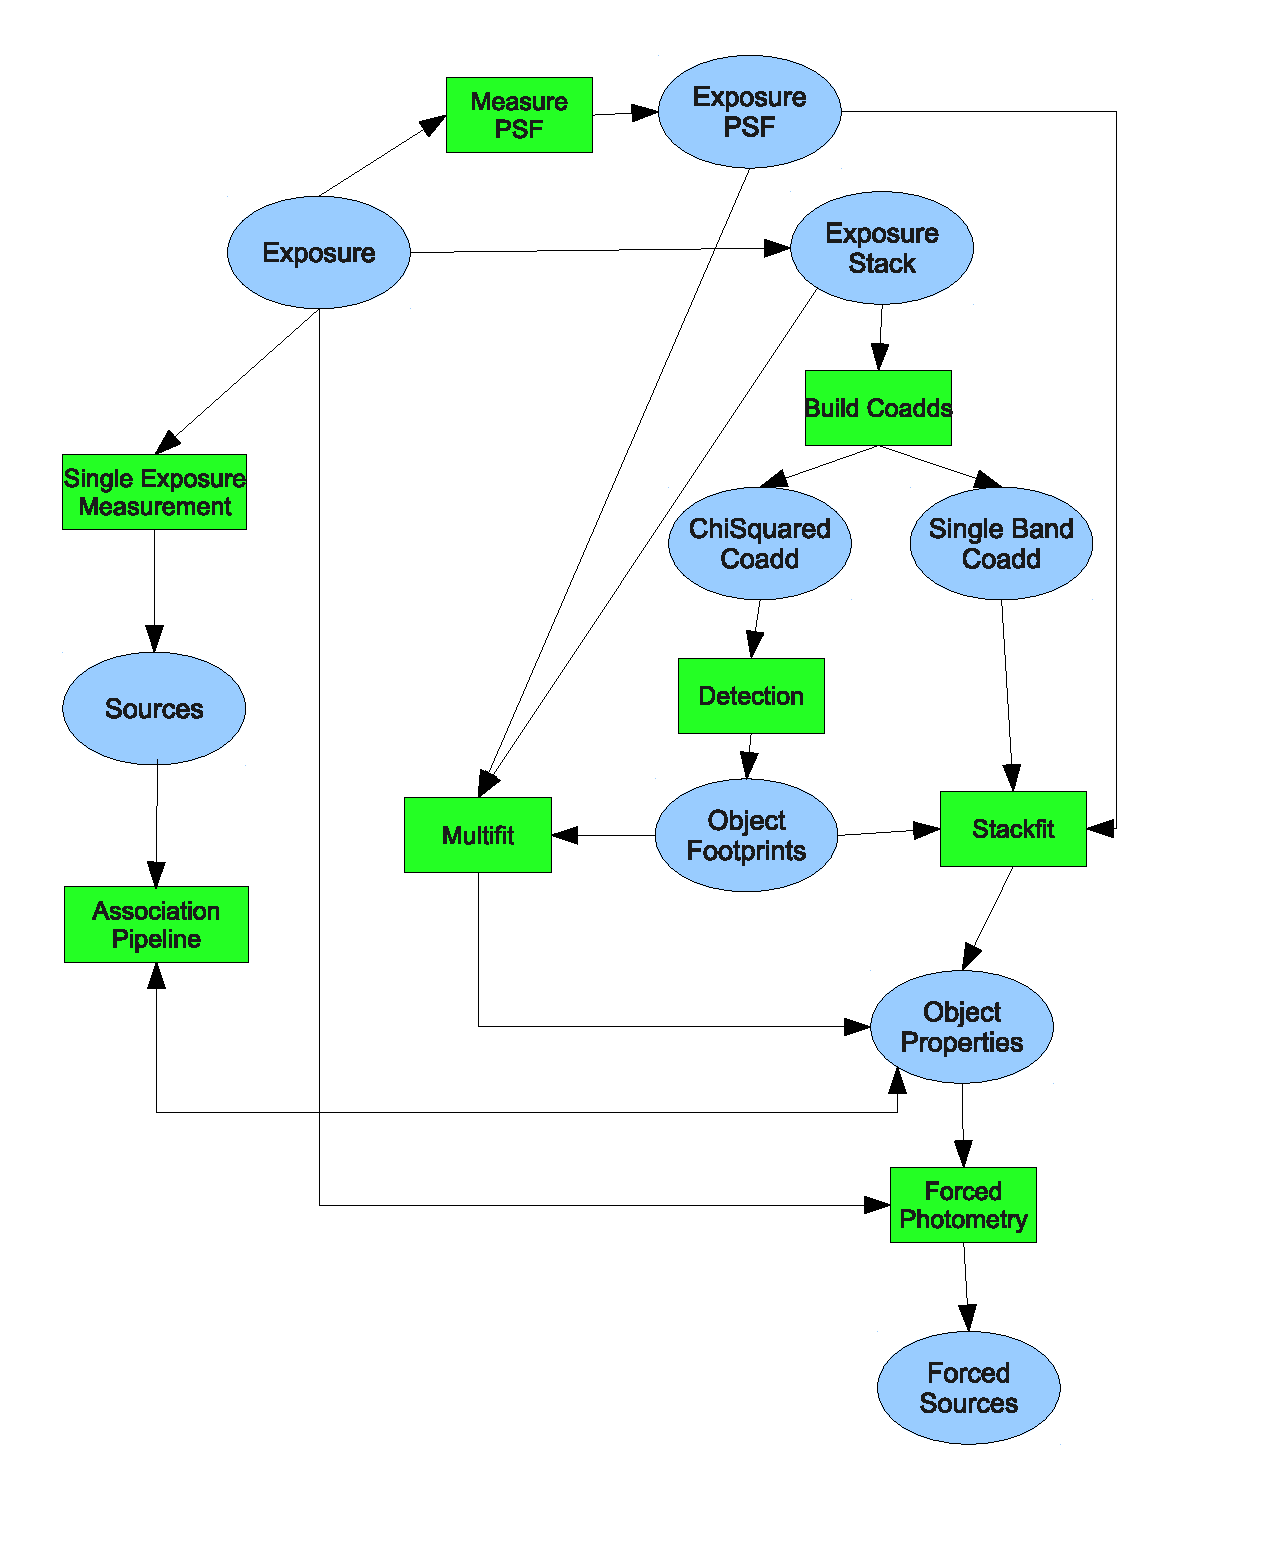
\includegraphics[angle=0,scale=0.75]{ObjectMeasurement.eps}
\caption{Processing flow for Object detection and measurement}
\end{figure}

\subsection{Object Detection}

% size of patches? what happens at edges? do patches need to overlap?
% note that patch size sets an upper limit to object size in the DB

\subsubsection{Single Exposure Measurement}
Objects that are bright enough to be detected at reasonable
signal-to-noise ratio in a single LSST Exposure are detected and
measured on a single Exposure basis. This processing utilizes traditional
crowded photometry techniques such as found in Dophot, DaoPhot, or
Sextractor.  This results in a set of Sources for each Exposure, which
are not initially associated with an Object.   This association is
performed subsequently by the Association Pipeline.

\subsubsection{Deep Detection}
The LSST science drivers depend on detecting and measuring Objects at
the full survey depth, approximately 3 mag fainter than the single
exposure depth.  To achieve this, the survey region is organized into
overlapping sky patches, and two types of deep coadded images are
created for each patch (see Section 6.3 for discussion of patch
size). The first, the ``chisquared'' coadd is formed from all
Exposures which contain the patch, regardless of filter band. It
measures each pixel's deviation from the local sky in a chi-squared
sense, and is used for object detection.  The second type is a coadd
of all overlapping exposures in a single filter band.  Care will be
taken to ensure that rapidly moving objects, such as Solar System
objects, do not appear in these coadds.  An object detection algorithm
is then run on the chisquared coadd, generating an initial Object
catalog.  An Object at this stage is nothing more than a pixel
footprint on the sky.  Measurements of object properties are still to
be performed, as discussed below.  At the end of the detection and
measurement process, an Object may have links to related Objects in a
segmentation tree that has been created by segmenting (deblending)
overlapping Objects.  The tree will be organized so that the root node
is the largest Object in the hierarchy, with the leaf nodes being the
smallest.  The segmentation algorithm to be employed is TBD, with
Sextractor or SDSS photo being examples of the kind of processing
involved.  The properties of the Objects that are segmented in this
way are then determined as discussed in the Measuring section below.
Note that later versions of the DMS may incorporate some aspects of
deblending into the measurement process, where better performance can
in principal be achieved.

\subsubsection{Difference Exposure Detection}
% include forced photometry on subset of objects
% note that DC part of AGN point source will not be separated from
% galaxy
% Have an example box here for AGN case?  and/or SN? explains the
% complex interplay between the three source types

New Objects may also be found during Difference Exposure processing. A
new Object will be created whenever a transient source which is detected in
the Difference Exposure from a Visit does not match any
Object already in the table.  The match will
take account of extendedness as well as position on the sky, so that a
new point source at the location of a galaxy already in the catalog
(for example, due to a supernova or variable AGN) will result in a new
Object.  This process is discussed further in the Example section below.

Note that this process cannot be perfect, since measuring the
extendedness of objects near the PSF size will always be uncertain.
Consequently, there will be cases where flux from a supernova or AGN
point source will be incorrectly added to the underlying galaxy rather
than to a new point source.  Between successive Data Releases,
however, these errors will decrease in number: as the survey goes
deeper, and accumulates images in better seeing, extendedness will be
better measured by the Object masurement procedure, as discussed in the
following sections.

\subsection{Object Characterization}

The DMS uses two separate approaches for measuring the properties of
faint Objects.  They are both model based, and the parameters of the
best fit model become the measured properties of the Object.  The two
approaches differ in how the models are fit to the pixels.  The
simpler approach, which we refer to as ``stackfit'', fits an Object
model to the single band coadd discussed in the previous section.  The
more sophisticated approach, which we refer to as ``multifit'' fits the
model simultaneously to all individual exposures of the Object in that
band.  The multifit approach will yield more accurate measurements,
particularly for more complex models, such as those which involve
motion.  It is far more expensive computationally, however, and cannot
be utilized for all Objects.  The DMS, therefore, will utilize
stackfit to measure \emph{all} Objects, while multifit will measure a subset of Objects that will
benefit the most from it, while keeping the computational cost within bounds. 

A high level view of the processing flow which generates Object
measurements from Exposures is shown in Fig. 7.  Note that both the
stackfit and multifit branches of the flow have the same end product:
For a given type of Object model, the parameters of the best fit model
become properties of the Object.  The model flux of the Object, and
its uncertainty, is determined for each individual Exposure in the
Exposure Stack which contains the Object pixels, resulting in a
ForcedSource for that Object in that Exposure.

We first discuss the two strategies for fitting Object models
to the pixels, and then the details of the models we employ.

\subsubsection{The Stackfit Algorithm}

The Stackfit algorithm follows the general approach laid out in Jee
and Tyson \citep{JeeTyson11}.  The PSF for each Exposure in the
Exposure Stack is carefully determined on an individual ccd basis.
This is necessary because the discontinuities in height and tilt
between ccds leads to discontinuities in the PSF which cannot be
accurately described by a smooth spatial model.  Note that the modeled
PSF is spatially varying within a given ccd.  For each Object, its PSF
is determined in the single band coadd by combining the PSFs measured
in the individual Exposures.  This allows an Object model, convolved
with that PSF, to be fit to the pixels in the single band coadd.
Then, for each Exposure in the Exposure Stack, the
best-fit model is convolved with the Object PSF for that Exposure, and
used to measure the Object flux in that Exposure, output as a ForcedSource. 

\subsubsection{The Multifit Algorithm}

The multifit approach is described in \citep{TysonAdass07}. The PSF is
determined on a per-Object, per-Exposure basis as with stackfit.
Instead of the Object model being fit to the single band coadd,
however, it is fit simultaneously to its pixel footprint in all
Exposures in the Exposure Stack for a given band, each Exposure being
convolved with its own PSF. Particularly for Objects with strongly
time-varying flux and/or significant motion on the sky, use of
multifit will result in more accurate models, and better flux
measurements at each epoch, at the expense of significantly greater
computational cost.  The choice of when to use multifit will be based
on heuristics that will evolve as the survey proceeds.

\subsubsection{Object Models}

Every Object is measured in the context of one or more object
models. Its measured properties include the model parameters which
generate the best fit of the model to the image pixels containing
the Object, and a covariance matrix
which quantifies the uncertainty in the fit.  When more than one model
can potentially apply to an Object, a fit for each model will be
determined.   In some
cases the correct model may not be clear from the fit results. For
example, a faint star with a significant proper motion may not be readily
distinguishable in the coadd from a galaxy with size slightly greater than the PSF
size.  This example, and numerous others, will be disambiguated as the
survey progresses, but some level of ambiguity will always remain. As
a further example, a small galaxy with a tidal tail will be poorly fit by
any of the models that we will employ.  For this reason, the DMS does
not choose between competing models, but makes all relevant results
available to science users. We anticipate that our initial set of
model types will evolve between data releases to take advantage of new
modeling approaches and our improving understanding of LSST data.  

Our choice of models for Objects is driven by astrophysics, by characteristics of
the LSST system, and by computing practicalities, as follows:

\begin{itemize}
\item Within the context of the LSST survey, clearly extended objects
  do not have measurable proper motion or parallax.  Comets are an
  exception, but they are processed only within difference
  exposures, not through Deep Detection. Supernova light echoes might also
  be an exception, and they deserve further thought.
\item While coadded exposures largely erase the effects of the gaps
  between the individual CCDs, individual exposures are strongly
  affected by them.  Processing of objects in individual exposures
  that extend across CCD gaps creates a significant overhead of
  programming complexity and computational cost, and will not
  initially be implemented in the DMS.  This capability can be
  incorporated in later versions of the DMS if it is warranted by the
  science gain.
\item Given the above constraint, model fitting is only useful if the
  object being fit is wholly contained within a single CCD field for
  the majority of the exposures in which it appears. Note that this
  does \emph{not} mean that an object needs to appear in the same CCD
  in different exposures!  This will rarely occur, given the survey's
  dithering pattern. If we want the object containment probability to
  be at least 0.8, the object size, $d$ can be no larger than $0.1~D$,
  where $D$ is the angular size of the CCD on the sky, 13 arcmin in
  the case of LSST.  This sets a natural upper limit on object size to
  be processed of approximately 1 arcmin.  We note that
  this size comfortably encompasses the objects required for the SRD's
  science drivers.
\end{itemize}

With that context, the initial model types are as follows:

\paragraph{Slowly Moving Point Source Model}

The Slowly Moving Point Source (SMPS) Model is intended to account for
the time varying fluxes and motion on the sky of point sources
(usually stars) with proper motions between zero and roughly 10
arcsec/yr. The model accounts for motion with respect to the local
astrometric reference frame that is generated by proper motion,
parallax, and possibly orbital motion with respect to a binary
companion.  When utilized by multifit, this model has the potential to
generate high quality astrometric models for faint sources. A similar
modeling and measurement approach has been successfully used by Lang,
Hogg, and Rix \citep{Lang08}.

The SMPS Model will be fit only to objects which are leaf nodes in the
segmentation tree.

\paragraph{Small Object Model}

The Small Object (SO) Model is intended to provide a robust
parameterization of small (diameter $<$ 1 arcmin) galaxy images for weak
lensing shear measurement and determination of photometric redshifts.
The final definition of ``diameter'' is TBD, but could plausibly be the 20
mag/arcsec$^2$ isophotal diameter, determined from the Detection Coadd.
The definition of the model flux profile is still TBD, but should
be driven by the needs of Photo-Z.  The measurement of the elliptical
shape parameters will be driven by the needs of weak lensing.  As with
the Point Source Model, each individual exposure generates either a
Source or a ForcedSource depending on the SNR.

The SO Model will be fit only to objects which are leaf nodes in the
segmentation tree.

\paragraph{Large Object Model}

A ``large'' object is one for which the 20 mag/arcsec$^2$ isophotal
diameter is greater than 1 arcmin, and less than 80\% of the patch
size (provisionally 13 arcmin, the CCD size).  This includes, for
example, the majority of NGC galaxies.  It is expected that the vast
majority of the science laid out in the SRD's four science drivers
will be accomplished with measurements made using the SMPS Model and
the SO Model.  But it is also recognized that there is much valuable
science, and numerous EPO applications, which will be based on larger
objects found in LSST images.  To at least partially satisfy this
need, large objects will have entries in the Object table, but will
not have any model fitting performed.  Thus, only some
columns of the Object table will contain measured properties of large
objects:

A typical large object will be segmented into smaller component
objects.  The leaf objects in the resulting segmentation tree will be
measured as described above, providing they qualify as ``small''.  The
large object itself, the root of the segmentation tree, will be
represented only by its ``Footprint'', with the following attributes: 

\begin{itemize}
\item Ellipse equivalent to Object footprint (same moments through second
order)
\item Footprint bounding box
\item Flux within footprint
\end{itemize}

Parameters resulting from model fitting, and from analysis of time
dependent properties, will be absent.  Fits of morphological models
(eg bulge/disk) to large objects must be created as Level 3 data
products.

Objects larger than ``large'' will not be represented in the DMS.

\paragraph{Solar System Object Model}
The predicted ephemerides from the orbit for a MovingObject
constitutes an object model which is used to measure the Object
in each exposure that contains the object, resulting in a ForcedSource.  
The details of the measurement process for Solar System Objects are not yet completely
defined. In particular, it is unclear if the measurements should be at
a position entirely fixed by the orbit prediction, or should be
allowed to compensate for prediction error by "peaking up" within some
error bound around the prediction.


\subsection{Model Residuals}

The measurement process can produce, in conjunction with every
Source or ForcedSource, a residual image that is the difference of the associated
image pixels and the pixels predicted from the model over the
footprint of the model.  Characterizing these residuals is important
for science such as strong lensing and merging galaxies, that will
identify interesting candidates for detailed analysis through their
residuals.  Selecting the most useful statistical measures of the residuals will
be the outcome of effort during the continuing design and development
phase of the project.

\subsection{An Example: Supernova in a Visible Galaxy}
As an example of the Object detection and maasurement process
discussed above, suppose that a supernova explodes in a ``small'' galaxy that is
clearly resolved in LSST imagery, and is already listed in the Object
table from a previous Data Release.  Suppose further that the
supernova is bright enough that it will be above the detection
threshold in at least one difference exposure.  The following sequence
of events will occur during the nightly Alert Production processing:

\begin{itemize}
\item The first time the supernova is detected above threshold in both
  difference exposures from a Visit, the Association Pipeline (AP) will
  attempt to match the resulting DiaSources to an Object in the Object
  table.  In this case, it will find that each DiaSource is contained
  within the footprint of its host galaxy, but based on the fact that
  the galaxy is extended, and the DiaSources are not, the AP will
  create a new Object (``SN'') at the position of the supernova
\item An Alert will be issued for the supernova.
\item On subsequent Visits, as long as the supernova remains above the
  detection threshold, new DiaSources will be created from each
  Exposure, and the AP will associate them to the SN object.   A query
  to the science database will readily retrieve all difference image
  photometry for SN from the DiaSources linked to the SN Object entry.
\item A likely policy for the survey to follow will be to add every
  Object that results in an Alert to a list of Objects to be force
  photometered in Difference Exposures. If this is done, the SN will
  result in ForcedSource entries even after it has dropped below the
  detection threshold above which it would generate DiaSources.   This
  will allow a query to the science database to retrieve this
  photometry as well.
\end{itemize}

When it is time to create a new Data Release, a new, empty, science
database is created.  It is populated with the Raw Exposures from the
survey extending from the inception of the survey up until the cutoff
date for the DR, but nothing else.  Note in particular that none of
the other Level 1 data products created by the Alert Production are
imported into the DR.  Processing always begins from scratch.  The
following sequence of events involving the supernova will thenoccur
during Data Release processing:

\begin{itemize}
\item As with all sky patches, a subtraction template coadd for each
  filter is created for the patch of sky containing the supernova by
  combining all the survey exposures that cover that patch. The
  combination algorithm strongly discriminates against transient flux,
  eg with a median.  The template coadd will therefore contain an
  image of the galaxy uncontaminated by the supernova.
\item A chisquared detection coadd is created for the patch of sky containing the
  supernova as discussed previously. The detection coadd contains
  floux from both the galaxy and
  the superimposed supernova.  The brightness of the supernova in the
  coadd depends on the fraction of the total coadd duration where the
  supernova has significant flux (so it becomes progressively fainter
  in subsequent DRs).
\item Object detection and deblending is run on the detection coadd.
  There are two cases to consider:
\begin{itemize}
\item The supernova is bright enough in the coadd to trigger
  deblending into a galaxy plus a point source (Case A). Three entries
  are made in the Object table: Gal+SN, Gal, and SN.  The Gal+SN
  object is the root of the segmentation tree, while Gal and SN are
  the deblended leaves.
\item The supernova is faint enough in the coadd that deblending is
  not triggered.  A single object is detected, with the galaxy flux
  slightly distorted by the supernova flux (Case B).  A single entry
  is made in the Object table: Gal*.  Gal* is not deblended, so it is
  a leaf node in the segmentation tree.
\end{itemize}
\item We will assume that the presence of a previous Alert has caused
  the DMS to choose this object for measurement by multifit.  Multifit
  is run on the exposure stack for the Objects entered into the table
  that are leaf nodes in the segmentation tree, two objects for Case
  A, one for Case B.  Given that Gal is ``small'', both the SO and
  SMPS models will be fit for these objects.  Let us consider Case A
  and B separately:
\begin{itemize}
\item For Case A, multifit is run separately on Gal and SN, fitting
  the SO and SMPS models for each.  The model residuals should clearly
  favor the SO model for Gal and the SMPS for SN, but note that the
  model parameters for both Gal and SN will be distorted by the
  presence of the other.  For example, the position of the SN/SMPS
  will appear to vary with time, since at low flux levels its profile
  will be significantly affected by the galaxy, but less so at high
  flux levels.  The Gal/SO position is not allowed to vary with time,
  by definition of the SO model, but its flux will vary due to the
  presence of the SN. [This argues that it is desirable to run
    multifit simultaneously on all models that overlap, or at least
    iteratively, subtracting models from the images. See Section 6.7]
  As a result of running multifit, ForcedSource entries will be generated
  for Gal at each epoch in the stack.  ForcedSource entries will also be
  generated for SN at each epoch.
\item For Case B, multifit fits both the SO and SMPS models to Gal*.
  The model residuals for the individual exposures will likely vary
  greatly with time.  If the Gal* was not deblended simply because the
  supernova occupied only a small fraction of the coadd time range,
  both SO and SMPS models will show large residuals, and in the case
  of SMPS, spurious motion as well.  Both Source and ForcedSource
  entries will be generated for Gal* at every epoch. 
\end{itemize}
\item With the multifit procedure complete, the difference exposures
  are formed by psf-matching and subtracting the template exposure
  from each exposure in the exposure stack.  By hypothesis, the
  supernova exceeds the detection threshold in at least some of these
  exposures.  For each exceedance, a DiaSource is created, and an
  attempt is then made to match it with an object already in the
  Object table just created by multifit.  Again, the outcome is
  different for Case A and Case B:
\begin{itemize}
\item For Case A, the DiaSources will match the SN object, and will be
  given that Object Id.
\item For Case B, the first DiaSource will not match Gal* because the supernova is a
  point source, while Gal* (by hypothesis) is measurably extended (it
  is also unlikely to match in position, but it may).  Therefore, a new
  Object is created for that DiaSource, call it SN*.  All subsequent
  DiaSources will then be associated to SN*.  
\end{itemize}
For both Case A and B, ForcedSource entries will be created for every
epoch in the stack by forced photometry on the difference exposures
%Note: this means that some ForcedSources will come from difference
%  exposures, some from science exposures
\end{itemize}

When the processing of the Data Release is complete, the following
information will be available for the supernova and its underlying
galaxy:
\begin{itemize}
\item Entries in the Object table for both the supernova and the
  galaxy.  For Case A, the model parameters reported for the supernova
  and the galaxy may each be significantly biased by the presence of
  the other
\item A full lightcurve for the supernova measured in difference
  exposures and reported in the ForcedSource entries associated with
  the supernova object
\item A full set of ForcedSources for the galaxy, each of which quantifies
  the residual between the model and the exposure from which the
  Source was measured
\item For Case A, a full set of ForcedSources for the supernova, each of
  which quantifies the residual between the model and the exposure
  from which the Source was measured
\item A partial set of DiaSources for the supernova, limited to those
  epochs where it is brighter than the detection limit
\end{itemize}
Note that the case of a time variable AGN embedded in a small galaxy
is broadly parallel to the supernova case considered above. Unlike the
supernova case, however, where the ForcedSources from difference
exposures give a nearly optimal extraction of the full light curve, in
the AGN case, only the ``AC'' part of the AGN light curve will be so
measured.  Some ``DC'' part of the AGN lightcurve will be part of the
flux associated with the galaxy.

\section{Inserting Synthetic Objects into the DMS Pipelines}
Many LSST science programs will need to determine their detection
efficiency for particular classes of objects.  For example, a program
to determine the SNIa rate in various types of galaxies will need a
quantitative understanding of the probability that a SNIa will be
detected by LSST as a function of redshift, the probability that the
supernova will be correctly classified, and the probability that the
host galaxy will be correctly classified.  To achieve this, there is
little alternative to inserting at the pixel level synthetic supernova
events in sythethic galaxies, processing these through the DMS
pipeline, and then performing the appropriate science on the resulting
database.  This must be done in a way that ensures that the Science
Database rigorously isolates synthetic from real objects.

The outline of this capability is:
\begin{itemize}
\item LSST DM will provide a general facility to add synthetic objects
  to existing LSST exposures, fully taking into account the observed PSF
  and sky background for each exposure.  This will be done by making
  use of the LSST image simulator, ImSim, which will be provided the
  existing Exposure to use as a background, the PSF model, and a model
  for the Object to be added.  
\item Science teams that wish to ascertain their detection efficiency
  for a particular class of objects will supply a model for the object class.
\item One or more ``mini-DR''s will be created using the normal Data
  Release procedures, with appropriate synthetic objects added to the
  input exposures. Separate tables describing the synthetic objects
  will be maintained within the Science Database.  A mini-DR will span a limited
  area of sky and/or time so that the computational requirements are
  tractable.
\item The Science Database for each mini-DR will be maintained as a
  completely separate database from those of any other DR.
\end{itemize}




\section{Incorporation of User Analysis Modules}

Over time, we expect that certain user-developed analysis modules
or pipelines may be found to be of such
broad interest and utility to LSST community users that their 
authors may be willing to contribute them to the public LSST code repository.
The code will then be available for any LSST user to incorporate in their personal analyses.
The project will welcome such contributions. 

It would be beneficial to LSST and all its users to streamline the process 
of code contribution, with special attention given to low-level basic tools 
that might be used by many groups.  Data Management will work to 
facilitate this by providing well-documented open-source interfaces, 
programming standards, and software quality metrics that external users can 
rely on in constructing their own pipelines and tools. 
Contributions which meet these standards will be eligible for 
inclusion in the project's code base. 
Data Management will provide a modest level of user support to assist users 
in meeting these requirements. 

There are some constraints, however: 
for instance, if contributed code brings in new external libraries or otherwise 
expands the dependencies of the code base, it may not be possible to include it. 
In addition, LSST may not be able to provide staff to support
non-trivial external code contributions in the long term.
We will encourage user groups to provide such support 
for their code, and will generally be willing to assist in this by making 
available the same support tools (such as for documentation and problem tracking) 
that we use in-house. 
User groups will be expected to produce documentation of the use and science data 
quality of contributed data products and code, 
and to take responsibility for its robustness when applied at LSST scales.

A possible final stage of the incorporation of contributed code would be for it 
to become part of the standard LSST data production and used to generate 
public data products centrally. 
We expect that this will turn out to be desirable at some point in the life of 
the project for some subset of contributed code.
There are important caveats: this will not be possible if it significantly increases 
the CPU, memory, or archival storage requirements of the system beyond its baseline, 
unless those costs are covered in some way at the time of the decision. 
It will also require an explicit agreement on the part of the contributors to 
support their code for the long term or find funding to increase the central support 
resources. 
Finally, any contributed code incorporated into production will have to be 
demonstrated to be highly reliable and must be integrated in the standard SDQA system, 
with the contributor responsible for defining and implementing the necessary metrics. 
For non-trivial contributions a peer review of the quality assurance plan would be 
advisable.

%suck in glossary text from UML
\section{Glossary}

\paragraph{API}
Applications Programming Interface  
\paragraph{DAC}
Data Access Center
\paragraph{DAQ}
Data Acquisition
\paragraph{DMS}
Data Management System
\paragraph{DR}
Data Release.
\paragraph{EPO}
Education and Public Outreach
\paragraph{Footprint}
The set of pixels that contains flux from an object. Footprints of multiple objects may have pixels in common.
\paragraph{FRS}
Functional Requirements Specification
\paragraph{MOPS}
Moving Object Pipeline System
\paragraph{OCS}
Observatory Control System
\paragraph{Production}
A coordinated set of pipelines
\paragraph{PSF}
Point Spread Function
\paragraph{RGB}
Red-Green-Blue image, suitable for color display.
\paragraph{SDS}
Science Array DAQ Subsystem.  The system on the mountain which reads
out the data from the camera, buffers it as necessary, and supplies it
to data clients, including the DMS.
\paragraph{SDQA}
Science Data Quality Assessment.
\paragraph{SMPS}
Slowly Moving Point Source model
\paragraph{SNR}
Signal-to-Noise Ratio
\paragraph{SO}
Small Object model
\paragraph{SQL}
Structured Query Language, the common language for querying relational databases.
\paragraph{TBD}
To Be Determined
\paragraph{Visit}
A pair of exposures of the same area of the sky taken in immediate
succession.  A Visit for LSST consists of a 15 second exposure, a 2
second readout time, and a second 15 second exposure.
\paragraph{VO}
Virtual Observatory
\paragraph{VOEvent}
A VO standard for disseminating information about transient events.
\paragraph{WCS}
World Coordinate System.  A bidirectional mapping between pixel- and sky-coordinates.

\begin{thebibliography}{10}

\bibitem{DMSSystem} \textbf{Data Management System Design}, 
https://www.lsstcorp.org/docushare/dsweb/Get/LDM-148, 2011

\bibitem{DMSFRS}  \textbf{Data Management Subsystem Requirements},
  https://www.lsstcorp.org/docushare/dsweb/Get/LSE-61, 2011

\bibitem{JeeTyson11} M. J. Jee and J. A. Tyson,  \textbf{Toward
  Precision LSST Weak-Lensing Measurement. I. Impacts of Atmospheric
  Turbulence and Optical Aberration}, PASP 123, 596(2011)

\bibitem{Lang08} D. Lang, D. Hogg, S. Jester, and H-W Rix,  \textbf{Measuring the undetectable: Proper motions and parallaxes of very faint sources}, ArXiv e-prints, 0808.4004 (2008)

\bibitem{MOPS} L. Denneau, J. Kubica, and R. Jedicke,
   \textbf{The Pan-STARRS Moving Object Pipeline}, Astronomical Data
  Analysis Software and Systems XVI ASP Conference Series, Vol. 376,
  proceedings of the conference held 15-18 October 2006 in Tucson,
  Arizona, USA. Edited by Richard A. Shaw, Frank Hill and David
  J. Bell., p.257

\bibitem{SRD}  \textbf{Science Requirements Document},
  https://www.lsstcorp.org/docushare/dsweb/Get/LPM-17, 2011 

\bibitem{SUI}  \textbf{LSST SUI Conceptual Design},
  https://www.lsstcorp.org/docushare/dsweb/Get/LDM-131, 2011

\bibitem{TysonAdass07} J. A. Tyson, et al,  \textbf{LSST and the
  Dark Sector: Image Processing Challenges}, Astronomical Data
  Analysis Software and Systems XVII O5.3, ASP Conference Series,
  Vol. 394 (2007)

\bibitem{WikiFedDB} Wikipedia,  \textbf{Federated database
  system}, http://en.wikipedia.org/wiki/Federated\_database, 2009.

\end{thebibliography}


\end{document}
